
\documentclass{article} % For LaTeX2e
\makeatletter
\def\input@path{{iclr/}}
\makeatother
\usepackage{iclr2027_conference,times}

% Optional math commands from https://github.com/goodfeli/dlbook_notation.
\input{math_commands.tex}
\renewcommand{\eqref}[1]{\textup{(\ref{#1})}}

\usepackage{url}
\usepackage{amsthm}
\usepackage{graphicx,booktabs,longtable,array,float}
\usepackage{hyperref}
\hypersetup{hidelinks}
\graphicspath{{iclr/}}
\newtheorem{proposition}{Proposition}
\newtheorem{lemma}[proposition]{Lemma}
\newtheorem{corollary}[proposition]{Corollary}
\DeclareMathOperator{\expit}{expit}
\DeclareMathOperator{\logit}{logit}
\DeclareMathOperator{\tr}{tr}
\newcommand{\RI}{\mathrm{RI}}



\title{Prediction and Uncertainty in Bayesian\\Survival Distillation}

% Authors must not appear in the submitted version. They should be hidden
% as long as the \iclrfinalcopy macro remains commented out below.
% Non-anonymous submissions will be rejected without review.

\author{Anonymous authors}



%\iclrfinalcopy % Uncomment for camera-ready version, but NOT for submission.
\begin{document}


\maketitle

\begin{abstract}
External survival models can provide useful information when target cohorts contain few observed events. We study generalized Bayesian survival distillation under fixed teacher guidance, combining a target survival likelihood, a prediction-level Kullback--Leibler loss, and a structural prior. We derive local responses of survival estimates and posterior means to deterministic teacher perturbations, and distinguish posterior curvature from the score variability governing repeated-cohort estimation. Simulations show that compatible guidance substantially improves neural survival prediction and reduces variability across target cohorts. Empirical interval coverage also improves relative to target-only fitting, although conditional-head intervals remain below nominal coverage. Imperfect teachers can still improve prediction at moderate borrowing strengths: the studied calibration shifts primarily affect absolute-risk accuracy, whereas risk-effect shifts also affect discrimination. Excessive reliance on a weak teacher can instead produce negative transfer relative to target-only fitting. Real-data analyses show improved pooled-reference recovery and potential benefit from borrowing between transplant populations, with direct teacher deployment remaining competitive. Together, these results connect the predictive benefits of survival distillation with the sensitivity and uncertainty of the fitted student.
\end{abstract}

\section{Introduction}
Survival prediction is often most difficult where reliable estimates are most needed. Local biomedical cohorts may contain only a few hundred patients, and rare events and censoring further limit the information available for fitting flexible models. Large registries and previously trained risk models can provide complementary information, but their individual-level training records may be inaccessible. Even when a source model is available, differences in covariates, parameterization, and architecture can prevent direct parameter transfer. Prediction-level methods address this limitation by reusing externally learned information without pooling source and target records \citep{hickey2024recast,lu2026adaptive}. Discrete-time survival knowledge distillation (DiSKD) combines a target survival likelihood with a Kullback--Leibler (KL) discrepancy between teacher and student predictions on target risk sets \citep{deng2026diskd}.

Accurate point predictions are only one requirement for clinical use. Patients with similar predicted risks may have substantially different levels of statistical support, particularly when target events are sparse or predictions rely heavily on external information. Uncertainty in individualized risk estimates matters for risk communication and decision support \citep{riley2025uncertainty,kompa2021second}. Kidney transplantation illustrates this setting: national registries contain extensive survival information, while a particular recipient population may provide relatively few events for local prediction \citep{salaun2024kidney}. We study uncertainty in patient-specific survival probabilities, conditional on a fixed deployed teacher, rather than uncertainty in the outcome of an individual patient or in retraining the external model.

A Bayesian formulation represents uncertainty over the student parameters and propagates it through the survival curve. However, teacher predictions do not constitute an additional independent sample. Unlike a power prior constructed from historical observations \citep{chen2000powerprior,ibrahim2015powerprior}, a distillation factor is evaluated on target subjects and their observed risk sets. We therefore formulate Bayesian DiSKD as a generalized update combining the target survival likelihood, a prediction-level teacher loss, and a teacher-independent Gaussian prior \citep{bissiri2016general,fang2024bkd}. The borrowing weight controls agreement with the teacher, while the prior scale controls structural regularization. The resulting posterior preserves the prediction-only transfer interface and the connection between the DiSKD objective and its posterior mode.

External guidance can improve prediction without being fully compatible with the target population. Differences in calibration, covariate effects, and source information can change both the value of borrowing and the direction in which it moves a student's predictions. Student capacity also matters: a representation unable to express the relevant covariate effects cannot necessarily recover them from an informative teacher. We analyze how deterministic teacher perturbations affect survival functionals and posterior means, linking the response to the local geometry of the student \citep{gustafson1996sensitivity}. This perspective separates the accuracy of the supplied teacher from the behavior of the student fitted under its guidance.

Borrowing also changes uncertainty, but posterior concentration and repeated-cohort stability are not interchangeable. A generalized posterior is governed locally by loss curvature, whereas the sampling variability of its fitted center also depends on subject-level score covariance \citep{miller2021,shaby2014,syring2019calibrating}. Consequently, improved coverage can accompany narrower intervals when borrowing improves centering and stability; conversely, concentration around a displaced center can leave coverage poor. In neural models, an additional distinction arises between a posterior over all student parameters and one that conditions on a learned representation. We keep these inferential targets separate throughout the analysis.

Our contributions are threefold. First, we formulate Bayesian DiSKD for censored single-event survival prediction and characterize local responses of student functionals to teacher guidance. Second, we distinguish posterior and sampling uncertainty, deriving an oracle benchmark that clarifies their different responses to borrowing. Third, we evaluate prediction and uncertainty under compatible and imperfect teachers, varying student architecture and target information. The simulations show substantial predictive benefits for neural students but persistent undercoverage of conditional-head intervals. Real-data studies complement these controlled comparisons through pooled-reference recovery in breast-cancer survival and transfer between kidney transplant populations, without treating estimated reference curves as individual-level truth.

\section{Related Work}
\paragraph{External borrowing and source-data-free survival transfer.}
Classical Bayesian borrowing methods assume access to historical observations or a compatible likelihood contribution. Power priors discount a historical-data likelihood, with a borrowing parameter controlling its influence \citep{chen2000powerprior,ibrahim2003optimality,ibrahim2015powerprior}. Prediction-level transfer instead uses a deployed model when source records or compatible parameters are unavailable. RECaST calibrates source predictions through a Bayesian random-effects formulation \citep{hickey2024recast}, while survival-transfer methods address heterogeneity between source and target populations \citep{lu2026adaptive}. DiSKD transfers survival information through predicted probabilities and a target likelihood \citep{deng2026diskd}. Our analysis concerns the resulting single-event student and conditions on the deployed teacher.

\paragraph{Knowledge distillation and Bayesian distillation.}
Knowledge distillation transfers predictive behavior for compression and data-efficient learning \citep{hinton2015distilling,gou2021survey}. Bayesian distillation connects teacher-informed probabilistic factors to student posteriors, MAP objectives, and uncertainty in class probabilities \citep{fang2024bkd}. Survival distillation adds censoring, time-indexed risk sets, and nonlinear survival functionals. We build on this probabilistic perspective rather than proposing Bayesianization of distillation alone: the focus is how target-dependent teacher losses affect the fitted survival curve and its uncertainty. Because the interface supplies fixed predictions, the posterior does not automatically propagate variability from the external training process.

\paragraph{Uncertainty in neural and clinical prediction.}
Dropout-based approximations and deep ensembles provide different approaches to uncertainty in flexible predictors \citep{gal2016dropout,lakshminarayanan2017deepensembles}. Their predictive usefulness does not make their uncertainty targets identical to a student posterior. In clinical risk prediction, the distinction between an estimated probability and uncertainty about that probability is important for interpretation and decision support \citep{riley2025uncertainty,kompa2021second}; transplantation provides a relevant application \citep{salaun2024kidney}. We study Bayesian uncertainty in survival probabilities and distinguish full-network inference from conditional-head inference. Relearning the representation across target cohorts introduces variation absent from a posterior that holds that representation fixed.

\paragraph{Generalized Bayes, sensitivity, and covariance calibration.}
Generalized Bayesian updating allows a task-specific loss to contribute to inference alongside a likelihood \citep{bissiri2016general}. Misspecified and generalized-posterior theory separates local posterior curvature from the sampling covariance of an estimator \citep{kleijn2012,miller2021}, motivating sandwich adjustments and calibrated credible regions \citep{shaby2014,syring2019calibrating}. Local Bayesian sensitivity expresses derivatives of posterior expectations through covariances with perturbations of the log density \citep{gustafson1996sensitivity}. We specialize these ideas to survival distillation, where the likelihood and teacher losses depend on the same patients. The resulting cross-covariance terms and the scope of the sampled parameters are essential to interpreting uncertainty; covariance adjustment alone cannot remove persistent prediction bias.

\section{Bayesian Discrete-Time Survival Knowledge Distillation}
\label{sec:method}
Bayesian DiSKD combines target outcomes and fixed prediction-level guidance in a generalized student posterior. The inferential targets are survival probabilities at specified covariates and horizons.

\subsection{Survival Student and Teacher Guidance}
\label{sec:model-interface}
Let $D=\{(X_i,Y_i,\Delta_i)\}_{i=1}^n$ contain independent subjects, with covariates, observed follow-up, and event indicators. On a fixed grid $0=t_0<\cdots<t_K$, let $A_{ik}$ indicate an observed at-risk interval and $\delta_i(t_k)$ an event in that interval. A student $f_\theta:\mathbb R^p\to\mathbb R^K$ defines hazards and survival probabilities by
\begin{equation}
\lambda_{\theta,k}(x)=\expit\{f_{\theta,k}(x)\},\qquad
S_\theta(t_k\mid x)=\prod_{\ell\le k}\{1-\lambda_{\theta,\ell}(x)\}.
\label{eq:survival-functionals-main}
\end{equation}
Cumulative event risk is $F_\theta=1-S_\theta$. A deployed teacher supplies fixed hazards $\widetilde\lambda_{ik}$, collectively $\widetilde P$, without requiring access to source records or matching teacher and student parameters.

Under the declared discrete observation model and conditionally independent censoring, the target likelihood is
\begin{equation}
L_{\rm tar}(\theta;D)=\prod_i L_i(\theta),\qquad
L_i(\theta)=\prod_k\lambda_{\theta,k}(X_i)^{A_{ik}\delta_i(t_k)}
\{1-\lambda_{\theta,k}(X_i)\}^{A_{ik}\{1-\delta_i(t_k)\}}.
\label{eq:target-likelihood-main}
\end{equation}
For continuous follow-up, this is a working discretization: censoring inside an interval is coded as a non-event in that occupied interval. Conditional independent censoring alone does not make this convention an exact continuous-time likelihood. Appendix~\ref{app:sim_design} specifies the encoding.

\subsection{Generalized Bayesian Distillation}
\label{sec:generalized-update}
The subject-level losses accumulate target evidence and teacher discrepancy on the same risk sets:
\begin{equation}
 r_i(\theta)=-\log L_i(\theta),\qquad
 q_i(\theta)=\sum_k A_{ik}\KL\{\operatorname{Bern}(\widetilde\lambda_{ik})
 \Vert\operatorname{Bern}(\lambda_{\theta,k}(X_i))\}.
\label{eq:subject-losses-main}
\end{equation}
Write $R_n=n^{-1}\sum_i r_i$, $Q_n=n^{-1}\sum_i q_i$, and $M_{n,\eta}=R_n+\eta Q_n$. With structural prior $\pi_\sigma=N(0,\sigma^2I)$, define
\begin{equation}
\Pi_{\eta,\sigma}(d\theta\mid D,\widetilde P)
\propto\exp\!\left[-\sum_i\{r_i(\theta)+\eta q_i(\theta)\}\right]\pi_\sigma(\theta)\,d\theta.
\label{eq:bayesian-diskd-posterior}
\end{equation}
The borrowing weight $\eta\ge0$ controls coupling to teacher predictions. The scale $\sigma$ controls structural shrinkage independently of the teacher. The teacher factor is constructed on target subjects, so it is a generalized update rather than an external-data likelihood \citep{bissiri2016general}.

\paragraph{MAP connection.}
Taking minus the log density and dividing by $n$ gives the penalized DiSKD objective $M_{n,\eta}(\theta)+\lambda_n\|\theta\|^2/2$, with $\lambda_n=(n\sigma^2)^{-1}$. Its minimizer is the posterior mode; posterior averaging defines the Bayesian predictor.

\subsection{Posterior Computation and Survival Summaries}
\label{sec:mala-inference-main}
Write $\theta=(\psi,w)$ for representation and prediction-head parameters, including intercepts. Full-state inference samples both blocks. In the main neural simulations, a separate MAP fit learns $\widehat\psi$ for each cohort and borrowing candidate, then \emph{conditional-head inference} freezes it and samples
\begin{equation}
\Pi_{\eta,\sigma}(dw\mid D,\widetilde P,\widehat\psi)
\propto\exp\!\left[-\sum_i\{r_i(\widehat\psi,w)+\eta q_i(\widehat\psi,w)\}\right]\pi_\sigma(w)\,dw.
\label{eq:head-posterior-main}
\end{equation}
This posterior conditions on the fitted representation; it differs from a full-network marginal. Full-state inference is retained for linear students and the real-data analyses explicitly identified below.

Starting near the MAP, the Metropolis-adjusted Langevin algorithm (MALA) uses exact full-data energies and gradients for the specified sampled parameters \citep{roberts1998}. Step sizes and preconditioners are adapted during warm-up and frozen for retained sampling. The simulation budget is four chains, 4,000 warm-up and 32,000 sampling iterations per chain, retaining 500 draws per chain; real-data budgets are reported separately. Acceptance calculations appear in Appendix~\ref{app:mala}. Each retained state induces a complete survival curve through Equation~\eqref{eq:survival-functionals-main}. For functional $\phi$, we report
\begin{equation}
\widehat\phi_B=\E_\Pi\phi,\quad\widehat\phi_B^{(M)}=M^{-1}\sum_m\phi(\theta^{(m)}),\qquad
\widehat I_{1-\gamma}(\phi)=[\widehat q_{\gamma/2},\widehat q_{1-\gamma/2}],
\label{eq:posterior-mean-main}
\end{equation}
where the finite-draw estimate approximates the posterior mean and quantiles use the functional draws. These are pointwise intervals for survival probabilities, not event-time predictions. We assess numerical error separately for posterior means, posterior SDs, interval endpoints, and predictive scores.

\subsection{Borrowing-Weight Selection by Target Prediction}
\label{sec:hyperparameters-main}
At fixed $\sigma$, the experiments select borrowing by target-likelihood widely applicable information criterion (WAIC) or refitted cross-validation (CV). To clarify subject deletion under this generalized posterior, define $\ell_i=\log L_i$ and $a_i=\ell_i-\eta q_i$. Deletion removes both terms. With teacher, prior, sampled parameters, preprocessing, grid, and remaining losses fixed,
\begin{equation}
\Pi_{-i}\propto\Pi\,e^{\eta q_i-\ell_i},\qquad
\mathrm{CPO}_i=\E_{\Pi_{-i}}L_i
=\frac{\E_\Pi e^{\eta q_i}}{\E_\Pi e^{\eta q_i-\ell_i}}.
\label{eq:cpo-main}
\end{equation}
The conditional predictive ordinates (CPOs) define $\mathrm{LPML}(\eta)=\sum_i\log\mathrm{CPO}_i(\eta)$, maximized over a prespecified grid including zero. We evaluate raw and Pareto-smoothed importance sampling (PSIS) estimates on METABRIC, reporting importance-weight diagnostics separately from posterior sampling diagnostics. Appendix~\ref{app:eta-algorithms} develops the formulation and explicit-refitting fallback \citep{vehtari2024}.

Conditional-head deletion keeps $\widehat\psi$ fixed; validation of the complete training procedure relearns representations and preprocessing within folds. Simulations select by WAIC over $\{1,2,3,5,10\}$, with $\eta=0$ a separate reference. Real-data candidates are $\{0,0.3,1,3,10\}$. Outer test outcomes never select the fitted model.

\section{Student-Functional Response and Uncertainty}
\label{sec:properties}
Teacher guidance changes both the center and spread of a fitted survival model. The following results characterize these effects for a fixed teacher and a specified set of sampled parameters. Full statements, assumptions, and derivations are in Appendices~\ref{app:formal-results}, \ref{app:local-regularity}, and~\ref{app:proofs}.

\paragraph{Teacher perturbations have functional-specific effects.}
Let $\theta_*(\varepsilon)$ minimize the expected penalized loss when teacher hazard logits are perturbed in a direction indexed by $\varepsilon$. Write $A$ for its Hessian at the baseline center, $B=\partial_\varepsilon\nabla_\theta Q$, and $g=\nabla_\theta\phi$ for a survival functional $\phi$. Under local smoothness and nonsingular curvature, Proposition~\ref{prop:functional-sensitivity} gives
\[
\phi\{\theta_*(\varepsilon)\}-\phi\{\theta_*(0)\}
=-\varepsilon\eta\,g^\top A^{-1}B+o(\varepsilon).
\]
Thus the same teacher change can affect patients and horizons differently. For fixed data, the corresponding posterior-mean response is
\[
\frac{d}{d\varepsilon}\mathbb E_{\Pi_\varepsilon}\phi
=-\operatorname{Cov}_{\Pi_\varepsilon}
  \{\phi,\partial_\varepsilon U_\varepsilon\},
\]
where $U_\varepsilon$ is the posterior energy (Corollary~\ref{cor:posterior-sensitivity}). This identity does not require a Gaussian posterior. These are local responses, not global monotonicity claims along a borrowing path.

\paragraph{Posterior concentration differs from sampling stability.}
Let $A$ be the curvature of the expected penalized subject loss and
$J=\operatorname{Var}\{\nabla r_i+\eta\nabla q_i\}$ its subject-score covariance.
For a locally regular identifiable model, Proposition~\ref{prop:local-spread-main} yields
\[
V_{{\rm post},\phi}\simeq\frac{g^\top A^{-1}g}{n},
\qquad
V_{{\rm samp},\phi}\simeq\frac{g^\top A^{-1}JA^{-1}g}{n}.
\]
The second expression is the sandwich variance. Because both losses use the same patient, $J$ includes their cross-covariance; adding teacher curvature alone does not determine sampling precision.

\paragraph{Oracle guidance supplies a transparent benchmark.}
With correctly specified observed-data hazards, an oracle teacher, and negligible first-order prior influence, the teacher score vanishes at truth. For identical Bernoulli risk-set contributions, Proposition~\ref{prop:oracle-spread} implies
\[
V_{{\rm post},\phi}/V_{{\rm samp},\phi}\simeq1+\eta.
\]
Both variances decrease with borrowing, but sampling variance decreases faster. This is a fixed-model oracle result, not a universal correction for neural intervals.

\paragraph{The fitting procedure defines the uncertainty target.}
Conditional-head intervals omit variation from relearning the representation, and fixed-hyperparameter covariance results omit variation from repeated selection. Moreover, spread is measured around the fitted population center, whose discrepancy from truth also affects coverage. These distinctions guide the experiments: predictive gains, repeated-cohort stability, and interval coverage are evaluated separately.

\section{Simulation Results}
\label{sec:experiments}

\subsection{Evaluation and fitting protocol}
\label{sec:exp_protocol}
Two single-event studies use the nonlinear survival law in Appendix~\ref{app:sim_design}, with twelve covariates and $K=20$ intervals. Independent target cohorts share a fixed teacher and analysis grid. Within each replicate, candidates use the same training and test subjects; the student, including its representation, is refitted for each candidate. Linear inference samples all coefficients and neural inference samples the conditional head. Gaussian scales are $\sigma=2$ and $0.25$, respectively. WAIC reselects $\eta$ over $\{1,2,3,5,10\}$ for selected-fit summaries; fixed-path comparisons do not reselect it. The target-only fit is a separate reference. Prior development is described in Appendix~\ref{app:prior-specification}.

Prediction metrics are concordance ($C^{\rm td}$), predictive deviance, integrated Brier score (IBS), integrated binary log loss (IBLL), and survival RMSE against the known law. At each fixed reference subject/horizon, EmpSD is the across-cohort SD of posterior-mean predictions and PostSD is the within-fit posterior SD. Post/Emp divides their reference-averaged SDs. Coverage and width concern pointwise 95\% intervals. Appendix~\ref{app:simulation-metrics} defines these metrics and distinguishes signed error from functional bias. Reported scores use binned follow-up; IBS and IBLL use marginal censoring weights and the terminal-bin convention specified in the appendix. Uncertainty comparisons and figure bands use paired cohorts.

All simulation fits enter the summaries. We assess numerical precision using $\widehat R\le1.05$, bulk effective sample size (ESS) $\ge200$, tail ESS $\ge100$, and endpoint Monte Carlo standard error (MCSE) $\le0.01$, monitored at 20 reference subjects and horizons $5,10,15$. These do not establish terminal-horizon precision. Appendix~\ref{app:convergence-results} separates numerical evidence from repeated-cohort coverage.

\subsection{Simulation I: Student behavior under compatible guidance}
\label{sec:sim1_results}
The oracle teacher supplies true interval hazards. The standard target cohort has $n=500$; we vary architecture, sample size, event frequency, and censoring while holding the teacher law fixed within each setting.

\paragraph{Prediction and representation.}
\label{sec:sim1_capacity}
Table~\ref{tab:sim1_architecture} compares target-only Bayesian fitting, the matched DiSKD point estimator, and Bayesian DiSKD across student architectures. Under the fixed prior and training protocol, compatible guidance substantially improves both discrimination and absolute-risk accuracy for the neural students. MediumMLP achieves the smallest survival error, whereas the linear student cannot represent the nonlinear covariate effects and remains close to chance discrimination. Thus an informative teacher is most useful when the student can express the information it supplies. The matched point estimates and posterior means have similar predictive performance; posterior sampling adds a distribution over survival curves rather than a uniformly superior point predictor.

The shared scalar-score TinyNN also benefits from guidance despite having an informative target-only fit. This supports a borrowing benefit beyond the weak target-only fits of the two MLPs. Architecture comparisons nevertheless change model structure as well as parameter count, so they do not isolate a dimension-only effect.



\begin{table}[!htbp]
\centering
\caption{\textbf{Simulation I: prediction under a compatible oracle teacher.} Entries are mean (standard deviation) across 100 paired cohorts for Linear, TinyNN, and SmallMLP and 50 for MediumMLP. Bayesian metrics are computed from posterior-mean survival curves. All methods within a student architecture use the same target cohorts; the oracle row summarizes direct predictions over the 100-cohort test set. Point estimates use the same structural penalty and posterior-selected borrowing weight. Linear inference is full-state; neural inference conditions on a separately fitted representation.}
\label{tab:sim1_architecture}\label{tab:sim1_architecture_full}
\footnotesize
\setlength{\tabcolsep}{4pt}
\begin{tabular}{llccccc}
\toprule
Student & Method & $C^{\rm td}\uparrow$ & Pred. dev. $\downarrow$ & IBS $\downarrow$ & IBLL $\downarrow$ & Surv. RMSE $\downarrow$ \\
\midrule
Linear & Target-only Bayesian & \shortstack{0.5044\\(0.0069)} & \shortstack{3.0111\\(0.0502)} & \shortstack{0.1508\\(0.0031)} & \shortstack{0.4664\\(0.0076)} & \shortstack{0.1884\\(0.0040)} \\
Linear & DiSKD point estimate & \shortstack{0.5007\\(0.0075)} & \shortstack{2.9705\\(0.0507)} & \shortstack{0.1498\\(0.0031)} & \shortstack{0.4639\\(0.0078)} & \shortstack{0.1849\\(0.0028)} \\
Linear & Bayesian DiSKD & \shortstack{0.5016\\(0.0075)} & \shortstack{2.9701\\(0.0507)} & \shortstack{0.1498\\(0.0031)} & \shortstack{0.4637\\(0.0078)} & \shortstack{0.1848\\(0.0028)} \\
\addlinespace
TinyNN & Target-only Bayesian & \shortstack{0.7521\\(0.0140)} & \shortstack{2.7502\\(0.0496)} & \shortstack{0.1204\\(0.0032)} & \shortstack{0.3875\\(0.0083)} & \shortstack{0.1015\\(0.0086)} \\
TinyNN & DiSKD point estimate & \shortstack{0.7937\\(0.0054)} & \shortstack{2.6269\\(0.0472)} & \shortstack{0.1099\\(0.0025)} & \shortstack{0.3525\\(0.0069)} & \shortstack{0.0399\\(0.0030)} \\
TinyNN & Bayesian DiSKD & \shortstack{0.7937\\(0.0054)} & \shortstack{2.6267\\(0.0472)} & \shortstack{0.1099\\(0.0025)} & \shortstack{0.3525\\(0.0069)} & \shortstack{0.0399\\(0.0030)} \\
\addlinespace
SmallMLP & Target-only Bayesian & \shortstack{0.5033\\(0.0157)} & \shortstack{3.0392\\(0.0454)} & \shortstack{0.1550\\(0.0030)} & \shortstack{0.4756\\(0.0068)} & \shortstack{0.2012\\(0.0059)} \\
SmallMLP & DiSKD point estimate & \shortstack{0.7934\\(0.0054)} & \shortstack{2.6360\\(0.0465)} & \shortstack{0.1102\\(0.0024)} & \shortstack{0.3555\\(0.0064)} & \shortstack{0.0449\\(0.0018)} \\
SmallMLP & Bayesian DiSKD & \shortstack{0.7934\\(0.0054)} & \shortstack{2.6366\\(0.0465)} & \shortstack{0.1103\\(0.0024)} & \shortstack{0.3557\\(0.0064)} & \shortstack{0.0454\\(0.0017)} \\
\addlinespace
MediumMLP & Target-only Bayesian & \shortstack{0.4986\\(0.0062)} & \shortstack{3.0089\\(0.0482)} & \shortstack{0.1507\\(0.0028)} & \shortstack{0.4662\\(0.0068)} & \shortstack{0.1890\\(0.0038)} \\
MediumMLP & DiSKD point estimate & \shortstack{0.7949\\(0.0053)} & \shortstack{2.6134\\(0.0453)} & \shortstack{0.1087\\(0.0023)} & \shortstack{0.3485\\(0.0064)} & \shortstack{0.0319\\(0.0046)} \\
MediumMLP & Bayesian DiSKD & \shortstack{0.7949\\(0.0053)} & \shortstack{2.6138\\(0.0453)} & \shortstack{0.1087\\(0.0023)} & \shortstack{0.3487\\(0.0064)} & \shortstack{0.0323\\(0.0047)} \\
\midrule
-- & Oracle teacher & \shortstack{0.7970\\(0.0053)} & \shortstack{2.5913\\(0.0476)} & \shortstack{0.1077\\(0.0024)} & \shortstack{0.3427\\(0.0070)} & \shortstack{0.0000\\(0.0000)} \\
\bottomrule
\end{tabular}
\end{table}

\paragraph{Target information and conditional uncertainty.}
\label{sec:sim1_difficulty}
Holding MediumMLP and the oracle teacher fixed, larger target cohorts improve prediction and reduce repeated-cohort variability (Table~\ref{tab:sim1_difficulty}). Heavy censoring modestly degrades performance relative to the standard setting. The low-event setting has smaller absolute survival errors, but its curves also lie closer to one; this should not be interpreted as greater information about rare events. Selected borrowing remains concentrated near the upper end of the candidate grid across these compatible-teacher settings.



Conditional posterior spread remains smaller than the empirical spread of the refitted predictions, and interval coverage remains well below nominal. The empirical distribution includes relearning the representation and selecting borrowing, whereas each posterior conditions on both. These results characterize the complete procedure's undercoverage; they neither test the fixed-model oracle variance ratio directly nor identify a single cause of the coverage gap.

\begin{table}[!htbp]
\centering
\caption{\textbf{Simulation I: target-data difficulty.} Selected $\eta$ is summarized by median [IQR]. SDs are calculated at each reference subject and horizon and then averaged; coverage and width are averaged within each cohort and then across cohorts. Parentheses give across-cohort standard deviations. Censoring percentages exclude administrative censoring, which accounts for the remainder after events and nonadministrative censoring.}
\label{tab:sim1_difficulty}\label{tab:sim1_difficulty_full}
\footnotesize
\setlength{\tabcolsep}{3pt}
\textbf{Target setting and selected borrowing}\par\smallskip
\begin{tabular}{@{}lcccc@{}}
\toprule
Scenario & $n$ & Event \% & Censor \% & Selected $\eta$ \\
\midrule
Standard & 500 & 29.8 & 20.2 & 10 [10, 10] \\
Small $n$ & 250 & 29.9 & 19.9 & 10 [10, 10] \\
Large $n$ & 1000 & 30.2 & 19.8 & 10 [10, 10] \\
Low event & 500 & 12.3 & 22.9 & 10 [10, 10] \\
High censor & 500 & 24.6 & 50.2 & 10 [10, 10] \\
\bottomrule
\end{tabular}
\par\medskip
\textbf{Prediction and conditional uncertainty}\par\smallskip
\begin{tabular}{@{}lcccccc@{}}
\toprule
Scenario & Signed error & EmpSD & Post/Emp & 95\% cov. & Width & Surv. RMSE \\
\midrule
Standard & \shortstack{$-0.0030$\\(0.0019)} & 0.0116 & 0.56 & \shortstack{0.3643\\(0.0234)} & \shortstack{0.0256\\(0.0028)} & \shortstack{0.0323\\(0.0047)} \\
Small $n$ & \shortstack{$-0.0055$\\(0.0032)} & 0.0160 & 0.51 & \shortstack{0.3393\\(0.0233)} & \shortstack{0.0318\\(0.0025)} & \shortstack{0.0427\\(0.0043)} \\
Large $n$ & \shortstack{$-0.0017$\\(0.0009)} & 0.0079 & 0.63 & \shortstack{0.4196\\(0.0242)} & \shortstack{0.0195\\(0.0014)} & \shortstack{0.0212\\(0.0028)} \\
Low event & \shortstack{$-0.0029$\\(0.0016)} & 0.0065 & 0.60 & \shortstack{0.3477\\(0.0231)} & \shortstack{0.0152\\(0.0015)} & \shortstack{0.0202\\(0.0020)} \\
High censor & \shortstack{$-0.0034$\\(0.0025)} & 0.0127 & 0.53 & \shortstack{0.3445\\(0.0193)} & \shortstack{0.0263\\(0.0035)} & \shortstack{0.0348\\(0.0055)} \\
\bottomrule
\end{tabular}


\footnotesize Each setting includes 50 cohorts. Convergence diagnostics are reported in Appendix~\ref{app:convergence-results}.
\end{table}

\paragraph{Variation across horizons.}
\label{sec:sim1_horizon}
Figure~\ref{fig:sim1_horizon} examines where along follow-up the aggregate gains arise. Borrowing improves prediction and coverage at every evaluated horizon, with moderate fixed borrowing generally between target-only and selected fits. The remaining coverage gap is especially pronounced late in follow-up. This temporal pattern complements the architecture comparison: improved prediction and narrower intervals can coexist with inadequate uncertainty about the true survival curve.

\begin{figure}[!htbp]
\centering
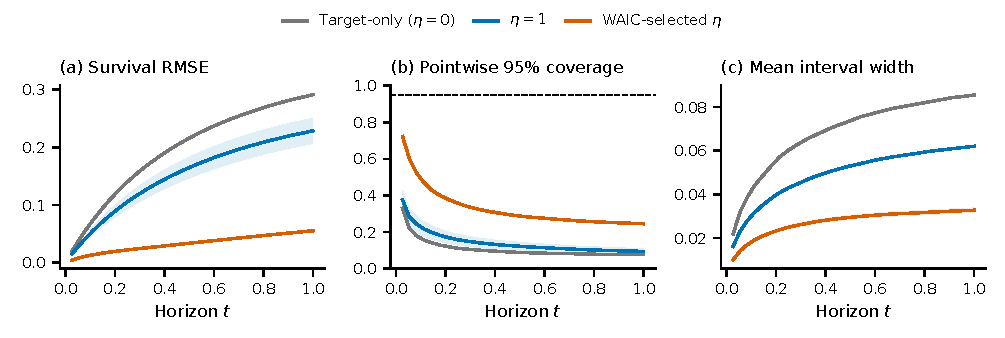
\includegraphics[width=\textwidth]{results/figures/fig1_horizon_rmse_coverage_width.pdf}
\caption{\textbf{Compatible guidance across horizons.} MediumMLP conditional-head RMSE, pointwise 95\% coverage, and interval width. Target-only, fixed $\eta=1$, and WAIC-selected fits each refit the representation per cohort/candidate. Bands are $\pm1.96$ cohort-mean MCSE over 50 paired cohorts; the coverage reference is 0.95.}
\label{fig:sim1_horizon}
\end{figure}

\paragraph{A low-dimensional reference.}
\label{sec:hj_results}
A low-dimensional, intrinsically discrete logistic example illustrates the oracle benchmark (Appendix~\ref{subsec:single_linear_control}). The functional variance ratio from inverse-Hessian and sandwich Gaussian draws increases approximately with the theoretical oracle ratio, alongside increasingly conservative posterior intervals. This comparison concerns covariance approximations rather than a matched full-network sampling experiment; its implementation limitations are documented in the appendix.
% PLACEHOLDER A: insert completed full-state control display here; see PENDING_VALIDATION.md.
% PLACEHOLDER B: insert completed fixed/refitted representation comparison in the uncertainty discussion, with details in the appendix.

\subsection{Simulation II: Student sensitivity to imperfect guidance}
\label{sec:sim2_results}
MediumMLP is paired with seven fixed teachers: estimated-compatible (10,000 external subjects), reduced-information (nine or six covariates), calibration-shifted (logit offsets 0.25 or 0.50), risk-shifted (different covariate effects), and small-external-cohort (250 subjects). Each regime uses 50 paired target cohorts. Teacher quality and selected prediction and uncertainty summaries appear in Table~\ref{tab:sim2_teacher_regimes_full}.

\begin{table}[!htbp]
\centering
\caption{\textbf{Simulation II: teacher regimes and selected Bayesian DiSKD performance.} Teacher metrics are evaluated against the target law on an independent reference sample. Selected $\eta$ is summarized by median [IQR] over candidates $\{1,2,3,5,10\}$. RMSE gain is target-only minus distilled-student RMSE; its parentheses give the Monte Carlo standard error of the paired difference. Other parentheses give standard deviations across cohorts.}
\label{tab:sim2_teacher_regimes}\label{tab:sim2_teacher_regimes_full}
\footnotesize
\setlength{\tabcolsep}{3pt}
\textbf{Teacher quality}\par\smallskip
\begin{tabular}{@{}lcccc@{}}
\toprule
Teacher regime & Teacher $R^2$ & Teacher RMSE & Teacher IBS & Teacher $C^{\rm td}$ \\
\midrule
Estimated compatible & 0.960 & 0.0365 & 0.1096 & 0.793 \\
Nine covariates & 0.510 & 0.1268 & 0.1281 & 0.699 \\
Six covariates & 0.216 & 0.1618 & 0.1407 & 0.622 \\
Calibration shift (mod.) & 0.910 & 0.0546 & 0.1100 & 0.794 \\
Calibration shift (sev.) & 0.744 & 0.0926 & 0.1168 & 0.791 \\
Risk shift (mod.) & 0.313 & 0.1523 & 0.1360 & 0.694 \\
Small external cohort & $-0.236$ & 0.2018 & 0.1557 & 0.503 \\
\bottomrule
\end{tabular}
\par\medskip
\textbf{Selected borrowing and target performance}\par\smallskip
\setlength{\tabcolsep}{2pt}
\begin{tabular}{@{}lccccccc@{}}
\toprule
Teacher regime & Sel. $\eta$ & $C^{\rm td}$ & \shortstack{Student\\IBS} & \shortstack{Student\\RMSE} & RMSE gain & 95\% cov. & Width \\
\midrule
Estimated compatible & 10 [10, 10] & \shortstack{0.7925\\(0.0060)} & \shortstack{0.1098\\(0.0028)} & \shortstack{0.0368\\(0.0027)} & \shortstack{0.1545\\(0.0006)} & \shortstack{0.3126\\(0.0170)} & \shortstack{0.0244\\(0.0020)} \\
Nine covariates & 2 [2, 3] & \shortstack{0.7458\\(0.0111)} & \shortstack{0.1218\\(0.0027)} & \shortstack{0.1074\\(0.0043)} & \shortstack{0.0839\\(0.0009)} & \shortstack{0.1428\\(0.0144)} & \shortstack{0.0381\\(0.0030)} \\
Six covariates & 3 [3, 3] & \shortstack{0.7075\\(0.0214)} & \shortstack{0.1312\\(0.0032)} & \shortstack{0.1383\\(0.0067)} & \shortstack{0.0531\\(0.0012)} & \shortstack{0.0862\\(0.0140)} & \shortstack{0.0315\\(0.0040)} \\
Calibration shift (mod.) & 10 [10, 10] & \shortstack{0.7927\\(0.0062)} & \shortstack{0.1102\\(0.0027)} & \shortstack{0.0494\\(0.0029)} & \shortstack{0.1420\\(0.0006)} & \shortstack{0.2249\\(0.0297)} & \shortstack{0.0262\\(0.0041)} \\
Calibration shift (sev.) & 2 [2, 5] & \shortstack{0.7899\\(0.0077)} & \shortstack{0.1138\\(0.0028)} & \shortstack{0.0783\\(0.0051)} & \shortstack{0.1131\\(0.0007)} & \shortstack{0.1434\\(0.0717)} & \shortstack{0.0386\\(0.0094)} \\
Risk shift (mod.) & 3 [2, 3] & \shortstack{0.7309\\(0.0136)} & \shortstack{0.1262\\(0.0038)} & \shortstack{0.1241\\(0.0086)} & \shortstack{0.0673\\(0.0014)} & \shortstack{0.1199\\(0.0159)} & \shortstack{0.0343\\(0.0035)} \\
Small external cohort & 1 [1, 1] & \shortstack{0.4993\\(0.0068)} & \shortstack{0.1516\\(0.0025)} & \shortstack{0.1908\\(0.0021)} & \shortstack{0.0005\\(0.0004)} & \shortstack{0.0864\\(0.0038)} & \shortstack{0.0452\\(0.0009)} \\

\bottomrule
\end{tabular}
\end{table}

\paragraph{Helpful and harmful borrowing.}
\label{sec:sim2_teacher_table}\label{sec:sim2_prediction_path}
Several imperfect teachers remain useful (Table~\ref{tab:sim2_teacher_regimes}). Estimated-compatible and moderately calibration-shifted guidance retain much of the oracle benefit, while reduced-information and risk-shifted teachers yield smaller gains. Selection generally favors stronger borrowing from informative teachers and intermediate weights from degraded teachers. The small-cohort teacher offers little improvement and selects the lowest positive candidate. Because the simulation grid excludes zero from selection, this boundary choice cannot be interpreted as an available no-borrowing decision.

\begin{figure}[!htbp]
\centering
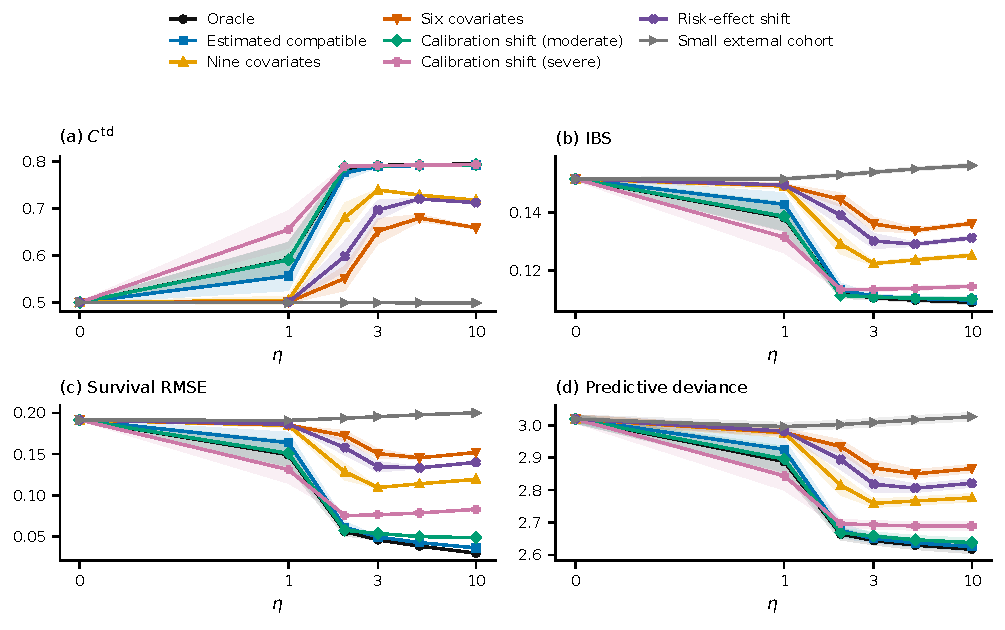
\includegraphics[width=\textwidth]{results/figures/fig3_teacher_eta_prediction_path.pdf}
\caption{\textbf{Prediction over the borrowing path.} MediumMLP conditional-head predictions for fixed teachers, with representations refitted per cohort/candidate. Means and $\pm1.96$ cohort-mean MCSE use 50 paired cohorts. Panels show concordance, IBS, survival RMSE, and predictive deviance; the $\eta$ axis is linear below one and logarithmic above.}
\label{fig:sim2_prediction_path}
\end{figure}

The fixed-weight paths reveal why the selected summaries differ (Figure~\ref{fig:sim2_prediction_path}). Severe calibration shift primarily harms absolute-risk accuracy while largely preserving discrimination: excessive borrowing worsens survival error relative to an intermediate weight, yet still improves on target-only fitting. Reduced-information and risk-shifted teachers also lose ranking information. By contrast, strong borrowing from the weak small-cohort teacher produces negative transfer relative to target-only fitting. Deterioration beyond an optimal positive weight and harm relative to no borrowing are therefore distinct phenomena.

\paragraph{Concentration under imperfect guidance.}
\label{sec:sim2_uq_path}
Increasing borrowing generally narrows intervals, but their centers depend on teacher compatibility. Calibration shifts can retain good discrimination while displacing survival estimates and reducing coverage. The supplementary uncertainty paths in Figure~\ref{fig:sim2_uq_path} show this distinction directly: teacher accuracy and posterior concentration alone do not determine interval reliability. These finite borrowing paths complement the local sensitivity analysis, which concerns a small perturbation at a fixed representation and borrowing weight.
% PLACEHOLDER D: predicted-versus-observed local responses, separate MAP and posterior mean, with MCSE; see PENDING_VALIDATION.md.


\section{Real-Data Experiments}
\label{sec:real-data}
We assess held-out prediction in a pooled-reference recovery study and an exploratory transfer between transplant populations. These are single-split analyses; a pooled model supplies estimated reference probabilities rather than individual truth.

\subsection{Recovery of pooled-data predictions: METABRIC}
\label{sec:real-pooled}
METABRIC contains breast-cancer follow-up with all-cause mortality \citep{katzman2018deepsurv}. An event-stratified split reserves 381 subjects for testing, 77 for target training (29 events within 120 months), and 1,446 for source training. The fixed teacher uses source records only; a separate pooled reference refits its architecture and source-selected regularization on source plus target-training records. Students have a 16-unit hidden layer, 20 interval outputs, and Gaussian scale $\sigma=1$. Bayesian inference samples all 500 parameters. All five final candidates pass the monitored functional criteria; Appendix~\ref{app:real-data} gives preprocessing, budgets, and diagnostics.

\begin{table}[!htbp]
\centering\footnotesize
\caption{\textbf{METABRIC prediction recovery.} Bayesian rows sample all 500 student parameters and report posterior-mean predictions. Generalized CPO, PSIS and complete five-fold refitting identify $\eta=10$ on the target-training data. Reference RMSE compares survival curves with the estimated pooled-data model. The matched-architecture DiSKD point baseline selects $\eta=3$ by its own target-training cross-validation. The complete Bayesian path and selector diagnostics appear in Appendix~\ref{app:real-data}.}
\label{tab:real-metabric}
\setlength{\tabcolsep}{4pt}
\begin{tabular}{@{}lccccc@{}}
\toprule
Method / $\eta$ & $C^{\rm td}\uparrow$ & Dev. $\downarrow$ & IBS $\downarrow$ & IBLL $\downarrow$ & Ref. RMSE $\downarrow$\\
\midrule
Teacher & .6699 & 3.3679 & .1363 & .4254 & --\\
Pooled reference & .6770 & 3.3549 & .1352 & .4224 & --\\
DiSKD point baseline & .6064 & 3.4575 & .1459 & .4524 & .1065\\
\midrule
Target-only Bayesian / $0$ & .6245 & 3.8674 & .1507 & .4576 & .1340\\
Bayesian DiSKD / $10$ & .6532 & 3.3948 & .1403 & .4342 & .0820\\
\bottomrule
\end{tabular}
\end{table}

Borrowing improves held-out target prediction and recovery of pooled-model survival curves (Table~\ref{tab:real-metabric}). The agreement between outcome-based scores and reference-recovery error supports the usefulness of prediction-level transfer in this small target cohort. The source teacher remains stronger on deviance and IBS. Bayesian DiSKD also improves on the separately tuned point baseline in this comparison, although their different penalties and selection procedures do not isolate the effect of posterior averaging.

Borrowing strength is chosen using target-training outcomes, excluding test subjects from both losses. Raw generalized CPO and PSIS estimates attain their maxima at $\eta=10$, also selected by complete five-fold refitting of the full network. All 25 CV fits meet the monitored numerical criteria. Importance-tail warnings indicate uncertainty in the case-deletion approximation; Appendix~\ref{app:real-data} reports these diagnostics and a target-likelihood WAIC sensitivity comparison. The selected weight is the upper endpoint of the prespecified grid.

The complete borrowing path is reported in Appendix~\ref{app:real-data}. Held-out deviance, IBS, and reference recovery favor the selected candidate, while discrimination and IBLL favor a neighboring weight. The evidence therefore supports borrowing without requiring every metric to rank the candidates identically. Test outcomes assess the selected model but do not enter its selection.



At the selected weight, survival intervals are narrower and pooled-reference inclusion is lower than under target-only fitting, although inclusion is not monotone along the borrowing path. Inclusion compares two estimated models and is not coverage of the true survival law.

\subsection{Transfer between kidney transplant populations}
\label{sec:real-kidney}
A teacher trained on 35,725 adult deceased-donor kidney-alone recipients is transferred to kidney--pancreas recipients in SRTR \citep{srtrSAF}. The single composite event is death or recorded kidney graft failure within one year. The target split has 1,935 training subjects (83 events) and 484 test subjects (21 events). At each weight, a new MAP fit learns the 16-unit representation; conditional-head inference then samples its 340 head parameters.

Moderate borrowing improves prediction relative to target-only fitting, but stronger borrowing does not improve all scores together (Table~\ref{tab:real-kidney}). In particular, better deviance can coincide with worse discrimination and integrated prediction scores. This resembles the imperfect-teacher simulation: the value of external information depends on both the borrowing strength and the aspect of prediction being evaluated. Direct teacher deployment remains competitive, so these results support local borrowing rather than a general advantage over the source model. The small number of test events limits comparisons, and interval-endpoint precision remains unresolved for the flagged candidates; all estimates are retained with their numerical qualifications.

\begin{table}[!htbp]
\centering\footnotesize
\caption{\textbf{Kidney-alone to kidney--pancreas transfer.} Scores use held-out target outcomes for the composite event. Bayesian rows are conditional-head posterior means at fixed borrowing weights. $\dagger$ marks fits that do not meet the interval-endpoint Monte Carlo precision criterion; their numerical estimates are retained rather than discarded. These are fixed-weight comparisons, not results of a validated selection procedure.}
\label{tab:real-kidney}
\setlength{\tabcolsep}{6pt}
\begin{tabular}{@{}lcccc@{}}
\toprule
Method / $\eta$ & $C^{\rm td}\uparrow$ & Dev. $\downarrow$ & IBS $\downarrow$ & IBLL $\downarrow$\\
\midrule
Teacher & .6157 & .6145 & .03356 & .14548\\
Target-only Bayesian / $0\dagger$ & .5835 & .9841 & .03995 & .21120\\
Bayesian DiSKD / $0.3\dagger$ & .5954 & .7802 & .04037 & .18205\\
Bayesian DiSKD / $1$ & .6089 & .6606 & .03451 & .14744\\
Bayesian DiSKD / $3$ & .5762 & .6445 & .03475 & .14981\\
Bayesian DiSKD / $10\dagger$ & .6607 & .6378 & .03381 & .14338\\
\bottomrule
\end{tabular}
\end{table}


\section{Discussion}
Compatible teacher guidance improves survival prediction in the studied configurations, with gains depending on the student's representation. Imperfect teachers can remain useful at moderate borrowing strengths. Calibration and risk-effect discrepancies affect absolute risk and discrimination differently, and excessive borrowing from a weak teacher can produce negative transfer.

The analysis connects these findings to two distinct quantities. Deterministic teacher changes induce functional-specific responses through the student's local geometry. Posterior curvature and patient-score covariance govern different notions of uncertainty; the correctly specified oracle case provides a transparent benchmark. Direct perturbation checks and a matched full-state comparison of posterior and repeated-cohort variance remain for future work.

The neural simulations evaluate conditional-head inference with representations refitted across cohorts. Coverage improves with compatible borrowing but remains below nominal, and the available comparisons do not isolate its causes. Real-data full-network and conditional-head results retain their distinct inference scopes. Predictive selection should be assessed through the selected model's predictions and numerical accuracy. Case deletion evaluates a specified conditional problem, while complete refitting evaluates the training procedure; prior development and sensitivity remain separate specification choices.


\section{Statements}
\subsection*{AI use statement}
Generative AI tools assisted manuscript drafting and editing, mathematical exposition, and research-code development and review.
% Authors should complete the disclosure of all other AI-assisted activities before submission.

\subsection*{Reproducibility statement}
Appendix~\ref{app:mala} describes posterior computation, Appendix~\ref{app:sim_design} specifies the simulation model and observation convention, and Appendix~\ref{app:proofs} gives proofs of the theoretical results.

\IfFileExists{iclr/references.bib}{%
  \bibliographystyle{iclr/iclr2027_conference}
  \bibliography{iclr/references}
}{%
  \bibliographystyle{iclr2027_conference}
  \bibliography{references}
}

\clearpage
\appendix


\section{Posterior Computation and Analysis Specifications}
\label{app:mala}

This appendix gives the MALA transition used in Section~\ref{sec:mala-inference-main} and the calculation of posterior survival summaries.

\subsection{Sampled state and exact energy}

For either choice of sampled parameters, the negative log target is
\begin{equation}
U_{\eta,\sigma}(\theta)=\sum_i\{r_i(\theta)+\eta q_i(\theta)\}+\|\theta\|^2/(2\sigma^2).
\label{eq:mala-energy-main}
\end{equation}

For a full-network analysis, $\theta$ contains every trainable student parameter, including the representation and interval-output parameters. For a frozen-feature analysis, the representation is held fixed and $\theta$ denotes only the sampled block. The latter posterior and its uncertainty are conditional on that representation. Teacher outputs, risk-set masks, the time grid, and $(\eta,\sigma)$ remain fixed throughout a run.

The Gaussian prior contributes once to the summed energy in Equation~\eqref{eq:mala-energy-main}. Equivalently, if an implementation evaluates mean losses, it must multiply their sum by $n$ before combining it with the prior energy. With a proper Gaussian prior and finite logits, the Bernoulli likelihood is positive and at most one, and $\exp(-n\eta Q_n)\in(0,1]$. The normalizing constant of Equation~\eqref{eq:bayesian-diskd-posterior} is therefore finite and positive. A formal flat prior establishes the MAP objective connection but does not by itself establish posterior propriety.

For $a_{ik}=f_{\theta,k}(X_i)$ and $p_{ik}=\expit(a_{ik})$, differentiation of the untempered losses gives
\begin{equation}
\nabla U_{\eta,\sigma}(\theta)
=\sum_{i,k}A_{ik}
\bigl[(p_{ik}-\delta_i(t_k))+\eta(p_{ik}-\widetilde\lambda_{ik})\bigr]
\nabla a_{ik}+\sigma^{-2}\theta.
\label{eq:neural-energy-gradient}
\end{equation}
This identity applies to the student parameterization and is useful for checking automatic differentiation and loss scaling. The teacher is not differentiated during student inference.

\subsection{Proposal and acceptance probability}

Let $B$ be symmetric positive definite and fixed during retained sampling. Define
\begin{equation}
\mu_\epsilon(\theta)
=\theta-\frac{\epsilon^2}{2}B\nabla U_{\eta,\sigma}(\theta),
\qquad
q_\epsilon(\theta'\mid\theta)
=\mathcal N\{\theta';\mu_\epsilon(\theta),\epsilon^2 B\}.
\label{eq:mala-kernel}
\end{equation}
For a proposed $\theta'$, accept with probability
\begin{equation}
a(\theta,\theta')=
1\wedge\exp\!\left[
-U_{\eta,\sigma}(\theta')+U_{\eta,\sigma}(\theta)
+\log q_\epsilon(\theta\mid\theta')
-\log q_\epsilon(\theta'\mid\theta)
\right].
\label{eq:mala-acceptance}
\end{equation}
Otherwise retain $\theta$ as the next state. Rejected transitions are part of the Markov chain and are not deleted from its posterior summary. Any adaptation of $\epsilon$ or $B$ is restricted to warm-up and frozen before retained transitions. Identity preconditioning is obtained with $B=I$.

For $p(\theta)\propto\exp\{-U_{\eta,\sigma}(\theta)\}$, the accepted flow satisfies
\[
p(\theta)q_\epsilon(\theta'\mid\theta)a(\theta,\theta')
=\min\{p(\theta)q_\epsilon(\theta'\mid\theta),
       p(\theta')q_\epsilon(\theta\mid\theta')\}.
\]
The symmetry of this expression gives detailed balance with the designated generalized posterior; the rejection probability supplies the remaining diagonal part of the transition. This establishes invariance of the target distribution by the standard Metropolis--Hastings argument \citep{roberts1998}.

Full-data energies and proposal gradients are evaluated consistently at both states. Exact accumulation of subject batches is compatible with this construction; substituting an uncorrected stochastic minibatch energy into Equation~\eqref{eq:mala-acceptance} is not the same transition. State-dependent preconditioning would also require its own correctly specified proposal, rather than the fixed-$B$ density above.

\subsection{Prediction and numerical assessment}

For each retained joint state, compute the complete vector of interval hazards and then the survival curve in Equation~\eqref{eq:survival-functionals-main}. Average those curves for point prediction and use their marginal quantiles for pointwise credible intervals. In general,
\[
\frac1M\sum_m\prod_{\ell\le k}(1-\lambda_{\theta^{(m)},\ell})
\ne
\prod_{\ell\le k}\left(1-\frac1M\sum_m\lambda_{\theta^{(m)},\ell}\right).
\]
Consequently, separately averaging parameters or hazards before constructing the survival curve is not the posterior-mean predictor. Likewise, pointwise intervals across horizons are not automatically a simultaneous band.

Convergence is evaluated using survival probabilities at the fifth, tenth, and fifteenth interval endpoints for 20 reference subjects. The $\widehat R$, effective sample size, and interval-endpoint Monte Carlo error thresholds are given in Section~\ref{sec:exp_protocol}. All fits remain in the experimental summaries, including those that fail one or more criteria.

Numerical convergence assesses approximation of the posterior for fixed data. Repeated-cohort evaluation assesses the statistical behavior of the fitted estimator and intervals. Sandwich-adjusted intervals use the latter covariance target.


\subsection{Numerical convergence and neural uncertainty}
\label{sec:numerical_audit_results}
\label{app:convergence-results}
Across the three neural architectures in the capacity comparison, 1,493 of 1,500 conditional-head fits satisfy all functional convergence criteria, compared with 320 of 1,500 full-network fits. For the five target-information settings, the corresponding counts are 1,438 and 66 out of 1,500. In Simulation~II, the oracle teacher and seven regimes in Table~\ref{tab:sim2_teacher_regimes_full} give 2,329 of 2,400 conditional-head passes (97.0\%) and 191 full-network passes (8.0\%). Each count includes $\eta\in\{0,1,2,3,5,10\}$. Most conditional-head fits meet the specified criteria, yet their intervals have low repeated-cohort coverage; full-network sampling remains computationally difficult.

For the five target-information settings, conditional-head convergence rates across all six borrowing weights are 97.7\% for the standard setting, 100\% for $n=250$, 82.7\% for $n=1000$, 100\% for low event frequency, and 99.0\% for high censoring. Each setting contributes 50 cohorts and 300 fits per sampled parameter block.

\section{Supporting Estimator and Prior Results}
\label{app:supporting-theory}
\subsection{Vanishing-borrowing expansion around the target law}
\label{app:vanishing-borrowing}

We next characterize how teacher borrowing and structural regularization can move the fitted center relative to the target law. Let
\begin{equation}
R(\theta)=\E\{r_i(\theta)\},
\qquad
\theta_0\in\arg\min_\theta R(\theta),
\qquad
Q(\theta)=\E\{q_i(\theta)\},
\label{eq:population-risks-main}
\end{equation}
and define
\begin{equation}
d_Q=\nabla Q(\theta_0),
\qquad
H_0=\nabla^2R(\theta_0).
\label{eq:target-gradient-main}
\end{equation}
Here $\theta_0$ is the target-only population optimum within the student model. If the student is correctly specified, it indexes the target survival law; under student misspecification, it is the corresponding target-model pseudo-true value. We call the teacher \emph{first-order compatible at $\theta_0$} when $d_Q=0$. This condition differs from training an estimated teacher under the same source and target event law, which still permits finite-sample estimation error. Calibration shifts, covariate-effect shifts, and other simulation perturbations are examples of mechanisms that may make $d_Q\neq0$; their effect enters through this score displacement.

\begin{proposition}[Target-centered local decomposition]
\label{prop:target-centered-main}
Suppose $R$ and $Q$ are twice continuously differentiable in a neighborhood of an identifiable interior minimizer $\theta_0$, $H_0\succ0$, the empirical gradients obey the usual uniform law and stochastic equicontinuity conditions, and $\eta_n\to0$ and $\lambda_n=(n\sigma_n^2)^{-1}\to0$. Let $\widehat\theta_n$ be a local minimizer of
\[
R_n(\theta)+\eta_nQ_n(\theta)+\frac{\lambda_n}{2}\|\theta\|_2^2
\]
that converges in probability to $\theta_0$. Then
\begin{equation}
\boxed{
\widehat\theta_n-\theta_0
=
-H_0^{-1}
\left[
\frac1n\sum_{i=1}^n\nabla r_i(\theta_0)
+
\eta_n d_Q
+
\lambda_n\theta_0
\right]
+
o_p\!\left(n^{-1/2}+\eta_n+\lambda_n\right).
}
\label{eq:target-centered-decomposition}
\end{equation}
\end{proposition}

Equation~\eqref{eq:target-centered-decomposition} separates three local contributions: target-cohort sampling variation, displacement induced by the teacher loss, and displacement induced by the structural prior. If $d_Q=0$, the teacher creates no first-order deterministic shift at the target-only optimum. If $d_Q\neq0$, the root-$n$ relevance of teacher mismatch is governed by $\sqrt n\,\eta_n d_Q$. The structural-prior contribution is governed by $\sqrt n\,\lambda_n\theta_0$; because $\lambda_n=(n\sigma_n^2)^{-1}$, its transition to first-order relevance occurs at
\begin{equation}
\sigma_n\asymp n^{-1/4}.
\label{eq:sigma-boundary-main}
\end{equation}
These are diagnostic asymptotic scales, not recommended universal schedules for selecting $\eta$ or $\sigma$.

\begin{corollary}[Target-centered posterior-mean survival functional]
\label{cor:posterior-mean-target-main}
Let $\phi(\theta)$ be a smooth identifiable survival functional with gradient $g_0=\nabla\phi(\theta_0)$. Under the conditions of Proposition~\ref{prop:target-centered-main} and a local posterior approximation for which posterior mean and local center differ by $o_p(n^{-1/2}+\eta_n+\lambda_n)$,
\begin{equation}
\widehat\phi_B-\phi(\theta_0)
=
-g_0^\top H_0^{-1}
\left[
\frac1n\sum_{i=1}^n\nabla r_i(\theta_0)
+
\eta_n d_Q
+
\lambda_n\theta_0
\right]
+
o_p\!\left(n^{-1/2}+\eta_n+\lambda_n\right).
\label{eq:functional-target-decomposition}
\end{equation}
\end{corollary}

The expansion separates target-sample fluctuation, teacher-induced displacement, and Gaussian-prior shrinkage when $\eta_n,\lambda_n\to0$. The projection $g_0^\top H_0^{-1}d_Q$ determines the first-order effect of teacher discrepancy on a particular survival functional. For finite fixed borrowing weights, Proposition~\ref{prop:functional-sensitivity} instead gives local derivatives around the current center.


\subsection{Supporting first-moment identity}
\begin{lemma}[First-moment preservation of the teacher loss]
\label{prop:first-moment-main}
At a fixed target risk-set cell, let $Q\in[0,1]$ be a random teacher event probability conditional on external data $D_{\rm ext}$, let $\bar Q=\E(Q\mid D_{\rm ext})$, and let $p_\theta\in(0,1)$. Then
\begin{equation}
\E\!\left[
\KL\{\operatorname{Bern}(Q)\Vert\operatorname{Bern}(p_\theta)\}
\mid D_{\rm ext}
\right]
=
\KL\{\operatorname{Bern}(\bar Q)\Vert\operatorname{Bern}(p_\theta)\}
+C_Q,
\label{eq:first-moment-main}
\end{equation}
where $C_Q$ does not depend on $\theta$.
\end{lemma}

Thus, when the teacher prediction is its predictive mean, that point prediction preserves exactly the student-dependent expected KL objective and its derivatives wherever they exist. The expected KL loss depends on the teacher distribution only through its mean, up to a parameter-independent constant.



\subsection{Conditions for the local estimator and posterior statements}
\label{app:local-regularity}

The local results concern a fixed teacher mapping, fixed time grid, fixed $\eta$, and a fixed-dimensional identifiable coordinate system; they do not assert global Gaussian behavior of an unrestricted neural network. Define $m_{i,\eta}=r_i+\eta q_i$, $M_\eta=R+\eta Q$, $\theta_\eta\in\arg\min_\theta M_\eta(\theta)$, and $b_\eta=\theta_\eta-\theta_0$, where $\theta_0$ minimizes the target risk $R$. Let $\lambda_n=(n\sigma_n^2)^{-1}\to0$ be deterministic, and set
\[
\theta_n=\arg\min_\theta\{M_\eta(\theta)+(\lambda_n/2)\|\theta\|^2\},
\qquad
\widehat\theta_n=\widehat\theta_{\eta,\sigma_n}^{\rm MAP}.
\]
Here and below a locally unique minimizing branch is used. The notation $\theta_{\eta,\sigma_n}$ elsewhere refers to $\theta_n$ and therefore may depend on $n$. The following are sufficient conditions for the stated local conclusions.
\begin{enumerate}
\item The population criterion is smooth near its interior minimizer, $\theta_n\to\theta_\eta$, and the empirical minimizing branch is consistent. The empirical Hessian converges uniformly on a neighborhood to its population counterpart. A locally Lipschitz Hessian supplies the $O(\lambda_n^2)$ population remainder.
\item The centered subject scores obey a central limit theorem at $\theta_n$, the required stochastic equicontinuity holds, and
\begin{equation}
H_n=\nabla^2M_\eta(\theta_n)+\lambda_nI\longrightarrow H\succ0,
\qquad
J_n=\Var\{\nabla m_{i,\eta}(\theta_n)\}\longrightarrow J.
\label{eq:fixed-pair-HJ}
\end{equation}
Subject-level covariance estimates and curvature estimates are consistent for these limits.
\item The generalized posterior concentrates on shrinking neighborhoods of $\widehat\theta_n$, admits a uniform local quadratic expansion there, and its rescaled law for $\sqrt n(\theta-\widehat\theta_n)$ converges to $N(0,H^{-1})$ with sufficient tail control. Convergence of posterior means and covariance additionally requires uniform integrability of the corresponding first and second rescaled moments. These moment conditions are not inferred from weak convergence alone.
\item A reported functional is twice continuously differentiable near the limiting target, with controlled Taylor remainder under that posterior concentration. Its projected sampling variance is positive when a standardized interval or variance ratio is used. The pointwise coverage corollary uses asymptotically Gaussian equal-tail quantiles.
\end{enumerate}

These conditions state the domain of the approximation \citep{vandervaart1998,chernozhukov2003,miller2021}. They must be checked for the estimating problem being analyzed. They need not hold uniformly when event information vanishes, the dimension grows, or neural parameter symmetries remain. Fixed-hyperparameter theory also does not automatically cover selection on the same target cohort.




\subsection{Prior specification and sample-size scaling}
\label{app:prior-specification}
For each simulation architecture, development compares $\sigma\in\{0.25,0.5,1,2\}$ using five independent standard-setting training/test pairs, each with 500 training and 5,000 test subjects. Candidates share each pair. Mean target-only MAP predictive deviance selects the scale: $2$ for Linear and $0.25$ for neural students. Each MAP fit uses four initializations, 300 Adam steps at learning rate $0.02$, then up to 300 L-BFGS iterations with strong-Wolfe search; the lowest-objective solution supplies predictions. The selected scale is frozen across target-information settings. Real-data students use $\sigma=1$. Neural scales lie at the lower boundary of the development grid. Both weights and intercepts are shrunk, but the existing results do not isolate intercept shrinkage as a cause of bias. No prior is retuned after inspecting coverage.

Three distinct specifications have different asymptotic meanings. A fixed prior keeps $\sigma$ constant and $\lambda_n=(n\sigma^2)^{-1}\propto n^{-1}$. A fixed average-loss penalty keeps $\lambda_n$ constant and requires $\sigma_n\propto n^{-1/2}$. A nonvanishing root-$n$ prior displacement occurs at $\sigma_n=c n^{-1/4}$, for which $\sqrt n\lambda_n=c^{-2}$. The oracle proposition instead requires $\sqrt n\lambda_n\to0$, equivalently $n^{1/4}\sigma_n\to\infty$. These are different regimes, not competing prescriptions.

Joint development selection, when specified, can minimize a target predictive score over a finite set of $(\eta,\sigma)$ pairs. It conditions the subsequent posterior on the chosen pair. Retrospective prior scales interpolated to attain simulation coverage use unavailable truth and do not define operational tuning. The rate analysis below is supplementary and does not change the priors used in the experiments.

\subsection{Asymptotic boundary of the structural-prior perturbation}
\begin{proposition}[Asymptotic boundary for structural regularization]
\label{prop:prior-scale-regime}
Under Appendix~\ref{app:local-regularity}, let $H_\eta=\nabla^2M_\eta(\theta_\eta)$ and suppose $\lambda_n\to0$. Then
\begin{equation}
\widehat\theta_{\eta,\sigma_n}^{\rm MAP}-\theta_\eta
=
-H_\eta^{-1}\left[
\frac1n\sum_{i=1}^n\nabla m_{i,\eta}(\theta_\eta)
+\lambda_n\theta_\eta
\right]+o_p(n^{-1/2}+\lambda_n).
\label{eq:prior-scale-expansion}
\end{equation}
Hence $\lambda_n=o(n^{-1/2})$ makes the structural-prior center shift first-order negligible; if $\sqrt n\lambda_n\to c\in(0,\infty)$, then
\begin{equation}
\sqrt n(\widehat\theta_{\eta,\sigma_n}^{\rm MAP}-\theta_\eta)
\Rightarrow
N\!\left(-cH_\eta^{-1}\theta_\eta, H_\eta^{-1}J_\eta H_\eta^{-1}\right),
\label{eq:prior-boundary-limit}
\end{equation}
and if $\sqrt n\lambda_n\to\infty$, the structural-prior displacement dominates root-$n$ sampling fluctuation unless its relevant directional coefficient vanishes. Because $\lambda_n=(n\sigma_n^2)^{-1}$, the transition is
\begin{equation}
\sigma_n\asymp n^{-1/4}.
\label{eq:sigma-quarter-rate}
\end{equation}
This is a diagnostic boundary for locally regular finite-dimensional or frozen-feature analyses, not a recommended universal prior schedule or neural-network coverage rule.
\end{proposition}



\subsection{Fractional-count interpretation and architecture invariance}
For a binary at-risk cell,
\begin{equation}
e^{-\eta\KL\{\mathrm{Bern}(\widetilde\lambda_{ik})\Vert\mathrm{Bern}(\lambda_{ik}(\theta))\}}
\propto
\lambda_{ik}(\theta)^{\eta\widetilde\lambda_{ik}}
\{1-\lambda_{ik}(\theta)\}^{\eta(1-\widetilde\lambda_{ik})},
\label{eq:pseudocountkernel}
\end{equation}
which yields the familiar DiSKD fractional-label interpretation. This is inherited from DiSKD and is included only as intuition for the teacher Gibbs factor.

\paragraph{Architecture invariance.}
Teachers giving identical probabilities on every target risk-set cell induce the same posterior for fixed data, student, prior, and borrowing weight, directly from Equation~\eqref{eq:subject-losses-main}.



\subsection{Local Gaussian interpretation of interval coverage}
\label{app:coverage}

Let $g=\nabla\phi(\theta_\eta)$ for a smooth scalar functional and define
\begin{equation}
v_{\rm post}=g^\top H^{-1}g,\qquad
v_{\rm samp}=g^\top H^{-1}JH^{-1}g>0.
\label{eq:coverage-variances}
\end{equation}
\begin{proposition}[Local Gaussian interval coverage]
\label{prop:functional-coverage}
Under Proposition~\ref{prop:local-spread-main} and the functional and moment conditions in Appendix~\ref{app:local-regularity}, suppose
\begin{equation}
\sqrt n\{\phi(\theta_n)-\phi_0\}\longrightarrow\delta.
\label{eq:local-functional-bias}
\end{equation}
Then the limiting coverage of a nominal $100(1-\gamma)\%$ equal-tail raw posterior interval for $\phi_0$ is
\begin{equation}
\Phi\!\left(\frac{z_{1-\gamma/2}\sqrt{v_{\rm post}}-\delta}{\sqrt{v_{\rm samp}}}\right)
-\Phi\!\left(\frac{-z_{1-\gamma/2}\sqrt{v_{\rm post}}-\delta}{\sqrt{v_{\rm samp}}}\right).
\label{eq:coverage-limit}
\end{equation}
If the limiting center is instead separated from $\phi_0$ by a nonzero amount and interval radius is $O_p(n^{-1/2})$, true-target coverage converges to zero.
\end{proposition}

This proposition separates local center bias and spread mismatch under the Gaussian approximation. Sandwich-adjusted intervals are reported separately from credible intervals of the original generalized posterior \citep{shaby2014,syring2019calibrating}.

\section{Additional Simulation Metrics and Results}
\label{app:simulation-metrics}
Predictive deviance is $-2m^{-1}\sum_i\log\E_\Pi L_i$ on $m$ independent test subjects. IBLL integrates the censoring-weighted binary score $-\{Z(t)\log S(t)+(1-Z(t))\log[1-S(t)]\}$ for survival status $Z(t)=\mathbb 1\{T>t\}$. Survival RMSE is the square root of the mean squared prediction error over subjects and horizons. Lower scores are better except for concordance. Pointwise coverage and width are averaged within a cohort and then across cohorts. Functional SDs are calculated at fixed reference subjects/horizons before averaging; a ratio of these average SDs differs from an average variance ratio. Signed prediction errors can cancel and are not a measure of absolute functional bias.

\paragraph{Binned concordance and censoring-weighted scores.}
Let $d_i\in\{0,\ldots,K-1\}$ be the observed interval index and $s_{ik}=\widehat S_i(t_{k+1})$. The reported concordance compares an event subject $i$ with subject $j$ if $d_j>d_i$, or if $d_j=d_i$ and $j$ is censored. It counts $s_{i,d_i}<s_{j,d_i}$ as concordant, gives prediction ties one-half credit, and excludes same-interval event/event pairs. This score uses interval ordering and no censoring weights.

For IBS and IBLL, the evaluated sample supplies the marginal censoring Kaplan--Meier estimate
\[
\widehat G_k=\prod_{j\le k}\left(1-\frac{\sum_i\mathbb 1\{d_i=j,\Delta_i=0\}}{\sum_i\mathbb 1\{d_i\ge j\}}\right),\qquad \widehat G_{-1}=1.
\]
The implemented Brier contribution is
\[
\widehat{\mathrm{BS}}_k=\frac1N\sum_i\left[
\frac{\mathbb 1\{\Delta_i=1,d_i\le k\}s_{ik}^2}{\widehat G_{d_i-1}}
+\frac{\mathbb 1\{d_i>k\}(1-s_{ik})^2}{\widehat G_k}\right].
\]
IBLL replaces the squared losses by $-\log(1-s_{ik})$ and $-\log s_{ik}$. Predictions are clipped to $[10^{-12},1-10^{-12}]$ and censoring denominators floored at $10^{-12}$. Trapezoidal integration uses $t_1,\ldots,t_K$, divided by $t_K-t_1$. Subjects censored in the evaluated interval contribute zero; at the final index every censored subject contributes zero. These are the binned scores used in the reported comparisons, including real data. Their terminal-interval convention differs from evaluation retaining exact censoring times. Marginal weights require censoring independent of predictors and event time, a stronger condition than conditional independent censoring alone.

Complete prediction and teacher-quality comparisons are reported in Tables~\ref{tab:sim1_architecture}, \ref{tab:sim1_difficulty}, and~\ref{tab:sim2_teacher_regimes}. The supplementary borrowing-path figure below resolves signed error, coverage, and interval width across fixed teacher regimes.







\begin{figure}[t]
\centering
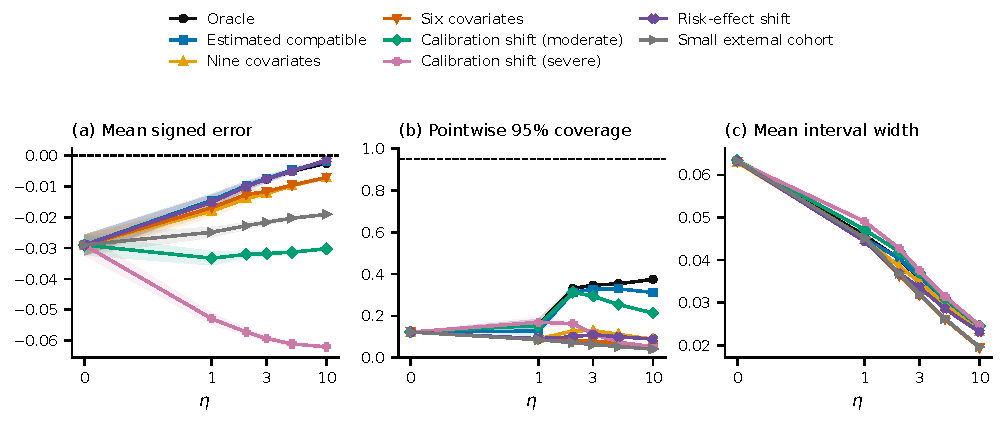
\includegraphics[width=\textwidth]{results/figures/fig4_teacher_eta_uq_path.pdf}
\caption{\textbf{Simulation II: conditional uncertainty over the fixed borrowing path.} Panels show mean signed survival error, empirical pointwise 95\% coverage, and mean 95\% posterior-interval width. Dashed references mark zero signed error and 0.95 coverage. Intervals condition on the fixed teacher, fitted representation, and indicated borrowing weight.}
\label{fig:sim2_uq_path}
\end{figure}

\section{Single-Event Oracle Reference}
\label{subsec:single_linear_control}
The low-dimensional model has $X\sim N(0,I_3)$ and intrinsic discrete event times, with administrative censoring after $K=10$ intervals. Its full student state consists of ten interval intercepts and three regression coefficients:
\begin{equation}
\operatorname{logit}\lambda_{0k}(X)=\alpha_k+X^\top\beta,
\qquad \beta=(0.8,-0.6,0.5)^\top.
\label{eq:simple_true_hazard}
\end{equation}
The intercept is $\alpha_k=-1.7346$, approximately $\logit(0.15)$. Administrative censoring occurs after the final interval.

\subsection{Gaussian and sandwich approximations}
\label{sec:e3_godambe}
We fit the single-event logistic model with $n=500$, $\sigma=10$, 20 independent cohorts, and 2,000 fixed reference subjects. The borrowing grid is $\eta\in\{0,0.25,0.5,0.75,1\}$. Each fit uses 2,000 AdamW steps and 3,000 Gaussian draws centered at the optimizer output. Raw covariance is the inverse summed Hessian including prior precision; sandwich covariance uses the patient-score second moment $\sum_i s_i s_i^\top$. This calculation uses the optimizer's default weight decay in addition to the explicit prior and an uncentered score estimate, so it provides an approximate reference for the covariance analysis.

\begin{table}[htbp]
\centering
\caption{Oracle Gaussian/Laplace approximation (20 cohorts). $\rho_V$ is the replicate mean of the ratio of reference-averaged functional variances from raw and sandwich draws.}
\label{tab:e3_global}
\begin{tabular}{@{}rrrrrr@{}}
\toprule
$\eta$ & Raw coverage & Sandwich coverage & Raw SD & EmpSD & $\rho_V$\\
\midrule
0 & 0.975 & 0.974 & 0.0277 & 0.0249 & 1.01\\
0.5 & 0.997 & 0.973 & 0.0225 & 0.0165 & 1.53\\
1 & 1.000 & 0.972 & 0.0195 & 0.0124 & 2.05\\
\bottomrule
\end{tabular}
\end{table}
The ratios of mean raw posterior SD to EmpSD are $1.11,1.36,1.57$. For raw and sandwich functional variances $v^{\rm raw}_{rjk}$ and $v^{\rm sand}_{rjk}$ at replicate $r$, reference subject $j$, and horizon $k$, the reported variance ratio is
\begin{equation}
\rho_V=\frac1R\sum_r\frac{\operatorname{mean}_{jk}v^{\rm raw}_{rjk}}
{\operatorname{mean}_{jk}v^{\rm sand}_{rjk}}.
\label{eq:legacy-functional-ratio}
\end{equation}
As borrowing increases, empirical sampling SD decreases faster than posterior SD. Sandwich adjustment reduces the additional conservatism while retaining coverage near 0.97.

\section{Simulation Design}
\label{sec:mechanism-experiments}
\label{app:sim_design}
The nonlinear experiments draw $X\sim N(0,I_{12})$ and define $Z_b$ as half the sum of covariates in block $b$ of four covariates. With target block coefficients $(b_1,b_2,b_3)=(2,2,8)$, the event rate is
\[
 r(x)=r_{\min}+\kappa\{(b_1Z_1)^2+(b_2Z_2)^2+2(b_3Z_3)^2\}.
\]
Conditional event times are exponential with rate $r(x)$, independent censoring times are uniform on $(0,c_{\max})$, and the administrative horizon is $1$. We set $r_{\min}=0.001$. In the standard setting, $\kappa=0.00432134$ and $c_{\max}=4.04788$. The low-event setting changes only $\kappa$ to $0.001220881014514313$; the high-censoring setting changes only $c_{\max}$ to $1.609697847336016$. Their calibration targets are observed-event fraction $0.12$ and nonadministrative censoring fraction $0.50$, respectively; realized fractions appear in Table~\ref{tab:sim1_difficulty_full}. The grid has 20 intervals, endpoints $0,1$, and 19 interior boundaries at quantiles $j/20$, $j=1,\ldots,19$, of observed event times ($T\le C,T\le1$) in an independent 200,000-subject standard-setting reference cohort. It is fixed across experiments. The true survival function is $S_0(t\mid x)=\exp\{-r(x)t\}$. Each replicate uses 5,000 independent test subjects, and uncertainty is evaluated on 2,000 fixed reference subjects.

Simulation I varies capacity and target information with an oracle teacher. Simulation II fixes MediumMLP and compares estimated-compatible, restricted-covariate, calibration-shifted, and risk-effect-shifted teachers. Capacity comparisons use 100 replicates for Linear, TinyNN, and SmallMLP and 50 for MediumMLP. Target-information and teacher comparisons use 50 replicates. Each borrowing path contains $\{0,1,2,3,5,10\}$; selection uses the positive candidates.

\paragraph{Student architectures.}
Linear uses interval intercepts and a shared linear covariate effect. SmallMLP has one hidden layer of width 16; MediumMLP has hidden widths 64 and 32. Both have SiLU activations and $K$ output logits. TinyNN has a width-8 hidden layer and a scalar output combined with interval-specific intercepts. Neural inputs contain all twelve covariates. Conditional-head inference conditions on the learned hidden layers and samples the output parameters.

\paragraph{Teachers and prediction quality.}
Estimated teachers use a shared scalar risk network with hidden widths 64 and 32 and interval-specific intercepts. The nine-covariate teacher observes $X_1,X_2,X_3,X_5,X_6,X_7,X_9,X_{10},X_{11}$; the six-covariate teacher observes $X_1,X_2,X_5,X_6,X_9,X_{10}$. Calibration shifts add $0.25$ or $0.50$ to the fitted estimated-compatible teacher logits. The risk-shifted source uses block coefficients $(5,0.5,3)$ in place of $(2,2,8)$, with its event fraction calibrated to the standard setting. For teacher survival predictions $\widetilde S_{jk}$ and true values $S_{0jk}$ on reference subjects $j$ and horizons $k$, we report
\[
R^2=1-\frac{\sum_{jk}(\widetilde S_{jk}-S_{0jk})^2}
{\sum_{jk}(S_{0jk}-\overline S_{0\cdot k})^2}.
\]
Each teacher mapping is fixed across target cohorts.

\paragraph{Partial-interval censoring convention.}
Observed follow-up is $Y=\min(T,C,\tau)$. We assign $Y$ to an interval and include that interval in the Bernoulli loss. For censoring strictly inside an interval, this convention records a non-event through its endpoint, whereas follow-up is observed only to $C$. It therefore approximates the continuous-time observation process. Oracle teacher probabilities remain the true full-interval hazards. The effect of this discretization on functional error is not isolated by the current experiments; the oracle benchmark instead assumes a correct discrete observation model.




% Source-only placeholders; the implementation handoff is PENDING_VALIDATION.md.
% Not empirical results. This file contributes no printed content.
% \section{Curvature and Sampling Variability Under Oracle and Shifted Guidance}
% \label{app:covariance-comparison}
% \emph{Results pending.} This comparison uses the logistic model in Appendix~\ref{subsec:single_linear_control}, with $n=500$, $K=10$, $\sigma=10$, administrative censoring, and 100 paired target cohorts. The oracle condition examines the spread comparison in Simulation~I, while the shifted condition distinguishes center displacement from spread error under the imperfect guidance studied in Simulation~II. The teachers are the true hazard and a fixed perturbation adding $0.5$ to its logit. Oracle fits use $\eta\in\{0,1,3\}$; shifted-teacher fits use $\eta\in\{1,3\}$ and share the target-only reference. MALA samples all thirteen parameters under the objective in Section~\ref{sec:method}.
%
% The comparison separates posterior SD estimated by MALA, inverse-Hessian SD, sandwich SD based on centered patient scores, and empirical SD across target cohorts. MAP and posterior-mean estimators have separate empirical SD estimates. The empirical variances of posterior means are also compared with their MCMC estimation variances. Bias is computed across cohorts at each fixed reference subject and horizon before taking its RMS across functionals. Table~\ref{tab:mechanism-spreads-main} summarizes horizons $2,5,10$; the full comparison retains all horizons.
%
% Coverage is evaluated against both the true survival law and the functional at the population minimizer of the penalized distillation objective, with $\lambda=(n\sigma^2)^{-1}$. Independent Gaussian quadrature over covariates and exact conditional integration over event times define this population reference. For score covariance, the integration retains each event outcome's random risk set. Raw intervals are MALA equal-tailed intervals. Adjusted intervals are MAP-centered functional Wald intervals with sandwich variance, intersected with $[0,1]$; MAP-centered curvature intervals provide a comparison with the same center and interval construction. Coverage of the penalized target distinguishes displacement from errors in estimating its sampling covariance.
%
% The likelihood, teacher, and symmetric cross-covariance contributions are projected onto the same functional gradients. Full-sandwich predictions are compared with empirical MAP variance and with predictions omitting the teacher or cross term. Under oracle guidance, the ratio of mean MALA functional variance to empirical estimator variance is reported separately for MAP and posterior means, alongside the finite-prior population approximation and the limiting reference $1+\eta$. Cohort-level resampling preserves pairing across borrowing weights when quantifying uncertainty in these comparisons.
%
% \begin{table}[htbp]
% \centering\scriptsize
% \caption{Estimator centers and raw posterior coverage in the logistic control. Results pending. EmpSD is evaluated separately for MAP and posterior-mean survival predictions; RMS bias refers to posterior means relative to truth. Raw coverage uses the same MALA intervals for the penalized population target $\phi_*$ and truth $\phi_0$. Table~\ref{tab:mechanism-spreads-main} gives the complementary spread and adjusted-coverage comparison.}
% \label{tab:covariance-comparison}
% \begin{tabular}{@{}lccccc@{}}
% \toprule
% Teacher / $\eta$ & RMS bias & \shortstack{EmpSD\\MAP} & \shortstack{EmpSD\\post. mean} & \shortstack{Raw cov.\\$\phi_*$} & \shortstack{Raw cov.\\$\phi_0$}\\
% \midrule
% Oracle / $0$ & -- & -- & -- & -- & --\\
% Oracle / $1$ & -- & -- & -- & -- & --\\
% Oracle / $3$ & -- & -- & -- & -- & --\\
% Logit shift $0.5$ / $1$ & -- & -- & -- & -- & --\\
% Logit shift $0.5$ / $3$ & -- & -- & -- & -- & --\\
% \bottomrule
% \end{tabular}
% \end{table}
%
% \section{Last-Layer Uncertainty With Fixed and Refitted Representations}
% \label{app:representation-uncertainty}
% \emph{Results pending.} In the nonlinear oracle setting with $n=500$ and $\eta\in\{0,10\}$, this comparison evaluates two training procedures over 20 paired target cohorts, using MediumMLP and $\sigma=0.25$. One learns a representation at $\eta=0$ from a single independent development cohort of size 500, holds it fixed across both borrowing weights and all target cohorts, and refits only the head. The other learns the representation anew from each target cohort and borrowing weight before conditional-head posterior sampling. Both optimize and sample the head conditional on their respective representations. The first procedure supplies a conditional-inference reference; its additional development data and representation quality preclude interpreting the comparison as a decomposition of representation variance.
%
% For each reference subject and horizon, the evaluation records bias, prediction RMSE, PostSD, EmpSD, coverage, interval width, and functional convergence diagnostics. Both procedures retain the observation convention used in Simulation~I. Their comparison examines the relation between conditional spread and repeated-cohort variability without attributing any remaining discrepancy to a single source of error.
%
% \begin{table}[htbp]
% \centering\scriptsize
% \caption{Last-layer uncertainty for fixed and refitted representations. Results pending. Bias is computed from the mean prediction across cohorts at each reference subject and horizon.}
% \label{tab:representation-uncertainty}
% \begin{tabular}{@{}lcccccc@{}}
% \toprule
% Representation & $\eta$ & RMS bias & RMSE & PostSD/EmpSD & Coverage & Width\\
% \midrule
% Fixed & $0$ & -- & -- & -- & -- & --\\
% Fixed & $10$ & -- & -- & -- & -- & --\\
% Refitted & $0$ & -- & -- & -- & -- & --\\
% Refitted & $10$ & -- & -- & -- & -- & --\\
% \bottomrule
% \end{tabular}
% \end{table}
%
% \section{Local Sensitivity of Posterior-Mean Survival Predictions}
% \label{app:teacher-sensitivity}
% \emph{Results pending.} The estimated-compatible teacher defines the baseline in Equation~\eqref{eq:teacher-perturbation}. The comparison retains Simulation~II's nonlinear data law, time grid, observation convention, MediumMLP student, $n=500$, and $\sigma=0.25$. We consider a calibration direction $d_k(x)=1$ and a direction toward the risk-shifted teacher, given by its logit difference from the baseline teacher, normalized to unit RMS over 2,000 independent development subjects and all horizons. The perturbations are $\varepsilon\in\{-0.1,-0.05,0,0.05,0.1\}$ at $\eta=3$, over ten paired target cohorts. The baseline posterior is shared by both directions. The difference between fitted teacher logits may include calibration and estimation effects as well as covariate effects.
%
% For each baseline fit, the representation remains fixed during conditional-head optimization and posterior sampling under every perturbation. We compare the predicted posterior-mean change
% \[
% \widehat\Delta_{\rm pred}
% =-\varepsilon n\eta\,\widehat{\operatorname{Cov}}_{\Pi_0}
% \{\phi,\partial_\varepsilon Q_n(\theta;0)\}
% \]
% with $\widehat\Delta_{\rm actual}=\widehat\phi_B(\varepsilon)-\widehat\phi_B(0)$. The MAP response $-\varepsilon\eta g^\top\widehat A^{-1}\widehat B$ is evaluated separately. Symmetric finite differences at both perturbation sizes provide an additional derivative comparison. Comparisons by horizon and perturbation size report response magnitudes and absolute approximation error together with Monte Carlo uncertainty. The posterior-mean response residual accounts for the dependence between its baseline mean and covariance estimate; small effects are retained even when they cannot be distinguished from Monte Carlo error. The main display uses horizons $5,10,15$, with all horizons retained for supplementary evaluation.
%
% The derivatives use the teacher probabilities in the implemented loss, including any numerical clipping. Functional predictions and covariance calculations use double precision. Additional MAP-only finite differences in $\eta$ and prior precision, with the same representation held fixed, assess Equation~\eqref{eq:hyperparameter-sensitivity} without adding another posterior-sampling grid.
%
% \begin{figure}[htbp]
% \centering
% \ResultFigurePlaceholder[0.14\textheight]{Posterior-mean response to teacher perturbations\\[4pt]\normalfont Results pending}
% \caption{Predicted and refitted changes in survival probability under a calibration offset and a perturbation toward the risk-shifted teacher, with the representation and distillation weight fixed.}
% \label{fig:teacher-sensitivity}
% \end{figure}
%
%
% \begin{table}[t]
% \centering\footnotesize
% \caption{\textbf{Posterior and sampling spread in the logistic control. Results pending.} Entries will average pointwise SD over fixed reference subjects and horizons $2,5,10$. EmpSD is the across-cohort SD of the MAP functional; PostSD is obtained from MALA. CurvSD and SandSD use the fitted-mode gradient and inverse-Hessian and sandwich covariances, respectively. The last coverage columns give coverage of MAP-centered sandwich intervals for the penalized population functional $\phi_*$ and the true survival probability $\phi_0$; $R$ records completed cohorts. Raw coverage, posterior-mean EmpSD, and RMS bias are reported in Appendix~\ref{app:covariance-comparison}.}
% \label{tab:mechanism-spreads-main}
% \setlength{\tabcolsep}{4pt}
% \begin{tabular}{@{}lccccccc@{}}
% \toprule
% Teacher / $\eta$ & \shortstack{EmpSD\\MAP} & PostSD & CurvSD & SandSD & \shortstack{Cov.\\$\phi_*$} & \shortstack{Cov.\\$\phi_0$} & $R$\\
% \midrule
% Oracle / $0$ & -- & -- & -- & -- & -- & -- & --\\
% Oracle / $1$ & -- & -- & -- & -- & -- & -- & --\\
% Oracle / $3$ & -- & -- & -- & -- & -- & -- & --\\
% Logit shift $0.5$ / $1$ & -- & -- & -- & -- & -- & -- & --\\
% Logit shift $0.5$ / $3$ & -- & -- & -- & -- & -- & -- & --\\
% \bottomrule
% \end{tabular}
% \end{table}
% \begin{table}[t]
% \centering\footnotesize
% \caption{\textbf{Simulation II: local functional response. Results pending.} RMS response errors compare predicted and refitted changes in survival probability, separately for the MAP and posterior mean. Each row combines $\varepsilon=\pm h$ over paired cohorts and fixed reference subjects at horizons $5,10,15$. RMS MCSE is $\{\operatorname{mean}(\mathrm{MCSE}_{\rm residual}^2)\}^{1/2}$, computed from pointwise posterior-mean response residuals with dependence between the baseline mean and covariance estimate retained. Uncertainty in the aggregate RMS error is assessed separately across cohorts. Horizon-specific comparisons and response magnitudes appear in Appendix~\ref{app:teacher-sensitivity}.}
% \label{tab:local-response-main}
% \setlength{\tabcolsep}{5pt}
% \begin{tabular}{@{}lcccc@{}}
% \toprule
% Direction & $h$ & \shortstack{MAP response\\RMS error} & \shortstack{Posterior-mean\\response RMS error} & RMS MCSE\\
% \midrule
% Calibration & $0.05$ & -- & -- & --\\
% Calibration & $0.10$ & -- & -- & --\\
% Toward risk-shifted teacher & $0.05$ & -- & -- & --\\
% Toward risk-shifted teacher & $0.10$ & -- & -- & --\\
% \bottomrule
% \end{tabular}
% \end{table}


\section{Real-Data Cohorts and Numerical Assessment}
\label{app:real-data}




\paragraph{Cohorts and preprocessing.}
Table~\ref{tab:real-cohorts} gives the analysis populations and event counts after administrative truncation. METABRIC and SUPPORT use the published preprocessed benchmark covariates; additional scaling is estimated within each training partition. The transplant cohorts include recipients aged at least 18 at deceased-donor transplantation between January 1, 2016 and December 31, 2018, without restricting transplant centers by volume. Kidney-alone recipients have no previous kidney transplant; no additional first-transplant restriction is imposed on kidney--pancreas recipients. Records with a kidney failure date before transplantation are excluded; kidney--pancreas records are also excluded if the pancreas failure date precedes transplantation. Pancreas failure itself is not an outcome in this analysis.

Follow-up starts at transplantation. The event date is the earlier recorded death or kidney graft-failure date, with events counted before 365.25 days. Graft failure uses the registry's recorded kidney failure date. When neither event date is available, censoring uses the last recorded patient-status date, truncated at one year. No source or target recipient lacks this status date, so the preprocessing fallback that assigns one-year follow-up when all follow-up dates are missing is unused. Reconstructing the endpoint from the dates reproduces every recorded event indicator and observation time. Day-zero events (178 source and six target recipients) are retained in the first interval. Missing numerical predictors are imputed using source-training means for the teacher and target-training means for the student; teacher predictions on target subjects retain the source transformations. Fixed categorical encodings follow the cohort definitions. Post-transplant dialysis variables and transplant-center indicators are excluded, leaving 127 covariates.

\begin{table}[htbp]
\centering\footnotesize
\caption{\textbf{Real-data analysis cohorts.} Event counts refer to the indicated analysis horizon. Transplant transfer uses distinct source and target populations; the other rows use within-cohort source/target splits.}
\label{tab:real-cohorts}
\setlength{\tabcolsep}{5pt}
\begin{tabular}{@{}lrrrrl@{}}
\toprule
Cohort & Source $n$ & Target train $n$ & Train events & Test $n$ (events) & Horizon\\
\midrule
METABRIC & 1,446 & 77 & 29 & 381 (139) & 120 months\\
SUPPORT & 6,743 & 355 & 173 & 1,775 (824) & 180 days\\
Kidney--pancreas & 35,725 & 1,935 & 83 & 484 (21) & 365.25 days\\
\bottomrule
\end{tabular}
\end{table}

\paragraph{Models and fitting.}
Teachers use a shared nonlinear score network with hidden widths 64 and 32 and interval-specific intercepts. Students use a 16-unit hidden layer and 20 interval-specific outputs. Teacher prior scale is selected by mean negative log likelihood on an event-stratified 20\% source-validation partition, then the teacher is refitted on the full source cohort. Candidate scales are $\{0.25,0.5,1\}$ for the benchmarks and $\{0.03,0.1,0.25\}$ for transplantation, selecting 0.25 and 0.03, respectively. Pooled references use the teacher architecture and selected scale, with their own pooled-training scaling and a Gaussian-penalized likelihood MAP fit. Bayesian student scale is fixed at 1, rather than the neural simulation scale 0.25. The priors, sample sizes and sampled parameter blocks therefore differ from the simulations; we compare qualitative prediction behavior, not matched posterior variance ratios. Full-network inference samples 500 parameters for METABRIC and 580 for SUPPORT. The transplant model has 2,388 parameters, of which 340 are sampled under conditional-head inference. No posterior temperature or interval recalibration is applied.

The shared grid has endpoints zero and the administrative horizon, with interior boundaries at the 19 empirical quantiles of source event times inside that horizon. An equidistant fallback is used if quantile boundaries coincide. As in the continuous-time simulations, censoring inside an interval is encoded as a non-event in that interval. IBS, IBLL, and concordance use the binned definitions in Appendix~\ref{app:simulation-metrics}. IBS and IBLL use marginal Kaplan--Meier censoring weights estimated on the test sample. These weights are used only for evaluation, not model fitting. They assume censoring independent of both event time and predictors; conditional independent censoring alone does not justify this marginal adjustment. Reference RMSE averages squared survival differences over test subjects and all 20 endpoints before taking the square root. Restricted mean survival time (RMST) is approximated by $\sum_{k=1}^{20}(t_k-t_{k-1})S(t_{k-1}\mid x)$ through the cohort's administrative horizon; reference RMST error is its mean absolute difference from the pooled model across test subjects.

The matched-architecture DiSKD point baseline uses the original distillation loss with AdamW and weight decay $10^{-4}$. Five-fold target-training tuning first selects learning rate from $\{5\times10^{-4},10^{-3}\}$ and batch size from $\{32,128\}$ without borrowing, then selects $\eta$ on the same folds. Each fit uses at most 128 epochs with patience 5; final training uses the ceiling of the median selected stopping epoch. This is a point-estimation comparator with the same MLP, not a reproduction of the original Transformer architecture. The Gaussian-prior MAP is a separate summary of the Bayesian objective.

\begin{table}[htbp]
\centering\footnotesize
\caption{\textbf{Complete METABRIC full-network prediction path.} Every completed Bayesian candidate is retained. Reference errors compare posterior-mean predictions with the estimated pooled-data reference; RMST error is in months. Lower scores are better except for concordance.}
\label{tab:real-metabric-path}
\setlength{\tabcolsep}{6pt}
\begin{tabular}{@{}rcccccc@{}}
\toprule
$\eta$ & $C^{\rm td}$ & Dev. & IBS & IBLL & Ref. RMSE & Ref. RMST error\\
\midrule
0 & .6245 & 3.8674 & .1507 & .4576 & .1340 & 8.386\\
0.3 & .6458 & 3.5860 & .1452 & .4436 & .1089 & 7.294\\
1 & .6560 & 3.4565 & .1418 & .4360 & .0976 & 6.878\\
3 & .6591 & 3.4066 & .1404 & .4336 & .0883 & 6.301\\
10 & .6532 & 3.3948 & .1403 & .4342 & .0820 & 5.816\\
\bottomrule
\end{tabular}
\end{table}

\paragraph{Full-network numerical precision.}
METABRIC results use four chains, 8,000 warm-up and 512,000 sampling iterations per chain, retaining 16,000 draws per chain. All five fixed-weight fits pass the criteria in Section~\ref{sec:exp_protocol}; maximum $\widehat R$ is 1.00146, minimum bulk ESS is 5,541, and maximum endpoint Monte Carlo standard error is 0.00825. The corresponding cross-validation fits use 8,000 warm-up and 256,000 sampling iterations, retaining 8,000 draws per chain, with one doubled extension when required. Six of the 25 fits require extension; all pass, with maximum $\widehat R=1.00294$ and minimum bulk ESS 3,636. The complete cross-validation run takes 4.85 hours on two CPU cores. These diagnostics concern training-subject survival functionals at three horizons, not a proof of exploration of every network parameter.

\begin{table}[htbp]
\centering\footnotesize
\caption{\textbf{METABRIC borrowing criteria and pooled-reference inclusion.} WAIC uses the full target-training posterior, whereas CV refits after removing validation subjects from both loss terms. Estimated expected log predictive density (ELPD) is summed over all validation subjects. MCSE ranges describe individual fold scores, not a standard error for the difference between criteria or candidates. Width and inclusion use pointwise 95\% intervals across held-out subjects and the 20 analysis horizons.}
\label{tab:real-selection}
\setlength{\tabcolsep}{5pt}
\begin{tabular}{@{}rccccc@{}}
\toprule
$\eta$ & WAIC $\downarrow$ & CV ELPD $\uparrow$ & Fold score MCSE & Width & Ref. inclusion\\
\midrule
0 & 242.288 & $-168.164$ & .070--.106 & .6592 & .9932\\
0.3 & 265.554 & $-152.352$ & .074--.097 & .5714 & .9999\\
1 & 267.925 & $-143.472$ & .038--.067 & .4673 & .9997\\
3 & 264.559 & $-138.540$ & .028--.047 & .3552 & .9892\\
10 & 263.604 & $-136.676$ & .022--.039 & .2417 & .9186\\
\bottomrule
\end{tabular}
\end{table}

For a validation fold, the score is $\sum_i\log\widehat\mu_i$, where $\widehat\mu_i=M^{-1}\sum_m L_i(\theta^{(m)})$. Its first-order Monte Carlo error is estimated from chainwise batch means of $\sum_i\{L_i(\theta^{(m)})/\widehat\mu_i-1\}$, retaining posterior dependence between validation subjects. We do not treat folds with overlapping training sets as independent replications.

The teacher loss also depends on each target subject's observed risk set. At fixed hyperparameters and preprocessing, deleting subject $i$ from the generalized posterior changes its density by a factor proportional to $\exp\{-\ell_i(\theta)+\eta q_i(\theta)\}$, where $\ell_i=\log L_i$. Likelihood-only WAIC does not explicitly include the second term. This distinction, refitting preprocessing and representations, and the smaller training sets in five-fold CV preclude assigning their observed disagreement to representation conditioning alone.

\paragraph{Generalized case deletion on METABRIC.}
We reconstruct each subject's likelihood and masked teacher KL from the existing full-network draws, using the original teacher, target scaling and source-derived grid. The self-normalized raw and PSIS estimates implement Equation~\eqref{eq:cpo-estimate}; the scored outcome remains $L_i$. PSIS uses ArviZ 0.22.0 with subject-specific relative MCMC efficiency estimated from the inverse deletion ratios. With $M=64{,}000$ retained draws, the warning threshold is $\min\{1-1/\log_{10}M,0.7\}=0.7$ \citep{vehtari2024}. Importance ESS is $(\sum_m v_{im}^2)^{-1}$ for normalized smoothed weights, not the MALA ESS or a score MCSE. All subjects remain in the sums, including flagged observations.

Tables~\ref{tab:real-cpo-diagnostics} and~\ref{tab:real-selector-consequences} separate posterior computation from importance-reweighting diagnostics. Every full-network fit meets the monitored functional criteria, while every candidate has some importance-tail warnings. Raw and PSIS LPML are largest at $\eta=10$, as is refitted CV. The warnings concern the accuracy of finite-draw importance estimates, not the case-deletion identity or the predictive benefit of the fitted model. We retain all estimates with their diagnostics rather than discard candidates by a universal all-subject threshold. No exact neural deletion refits are used. Algebraic checks cover ordinary CPO at $\eta=0$, teacher-constant invariance, original-loss deletion, and direct deletion in an analytically tractable normal model. Reconstructed losses reproduce posterior energies and target-likelihood WAIC. This postprocessing takes 88.7 seconds on one CPU core, excluding environment preparation and tests.

\begin{table}[htbp]
\centering\footnotesize
\caption{\textbf{METABRIC posterior and case-deletion diagnostics.} The first panel reports worst-case diagnostics over monitored survival functionals. The second reports all raw/PSIS LPML estimates and importance diagnostics. Counts with $\widehat k\geq0.7$ indicate sensitivity of importance estimates, not candidate exclusion. Importance ESS is reported as minimum/median over the 77 subjects.}
\label{tab:real-cpo-diagnostics}
\setlength{\tabcolsep}{5pt}
\begin{tabular}{@{}rcccc@{}}
\toprule
$\eta$ & Max. $\widehat R$ & Min. bulk ESS & Min. tail ESS & Max. endpoint MCSE\\
\midrule
0 & 1.00145 & 5541 & 10502 & .00825\\
0.3 & 1.00041 & 7458 & 16565 & .00588\\
1 & 1.00068 & 11214 & 25261 & .00486\\
3 & 1.00067 & 10724 & 24551 & .00507\\
10 & 1.00083 & 8100 & 18064 & .00616\\
\bottomrule
\end{tabular}
\par\medskip
\begin{tabular}{@{}rcccccc@{}}
\toprule
$\eta$ & Raw LPML & PSIS LPML & Max. $\widehat k$ & $\widehat k\geq.7$ & $\widehat k\geq1$ & Importance ESS\\
\midrule
0 & $-153.804$ & $-149.018$ & 1.134 & 38/77 & 8/77 & 10.7 / 2941\\
0.3 & $-145.221$ & $-142.920$ & 1.017 & 28/77 & 1/77 & 27.4 / 5065\\
1 & $-137.993$ & $-137.196$ & .880 & 17/77 & 0/77 & 130.6 / 13427\\
3 & $-133.406$ & $-133.120$ & .900 & 19/77 & 0/77 & 122.5 / 28562\\
10 & $-132.078$ & $-131.896$ & .917 & 15/77 & 0/77 & 90.2 / 33812\\
\bottomrule
\end{tabular}
\end{table}

\begin{table}[htbp]
\centering\footnotesize
\caption{\textbf{METABRIC borrowing-weight selection.} Scores rank candidates within a criterion, not different criteria against one another. WAIC is minimized; raw/PSIS LPML and CV ELPD are maximized. $*$ marks estimated importance-based maximizers with tail warnings.}
\label{tab:real-selector-consequences}
\setlength{\tabcolsep}{5pt}
\begin{tabular}{@{}lrcl@{}}
\toprule
Criterion & $\widehat\eta$ & Score & Numerical assessment\\
\midrule
Target-likelihood WAIC & 0 & 242.288 & All five fits meet monitored criteria\\
Raw CPO$^*$ & 10 & $-132.078$ & Tail warnings at every candidate\\
Generalized PSIS-LOO$^*$ & 10 & $-131.896$ & Tail warnings at every candidate\\
Complete five-fold CV & 10 & $-136.676$ & All 25 fits meet monitored criteria\\
\bottomrule
\end{tabular}
\end{table}

Raw CPO, PSIS, and complete cross-validation select the same fitted candidate and therefore have identical held-out predictions, reported in Table~\ref{tab:real-metabric-path}. The WAIC-selected candidate is the target-only fit. These comparisons are descriptive: uncertainty in test-score differences is not estimated, so close numerical ranks are not resolved.

\paragraph{Transplant numerical assessment.}
All five conditional-head fits require one extension of the initial four-chain budget, doubling warm-up from 4,000 to 8,000 iterations and sampling from 32,000 to 64,000 iterations, and halving the initial step size. Each final fit retains 1,000 draws per chain. At $\eta=0,0.3,1,3,10$, maximum endpoint Monte Carlo standard errors are respectively 0.0405, 0.0186, 0.0088, 0.0098 and 0.0120. All meet the $\widehat R$ and ESS thresholds, but only $\eta=1,3$ meet all four criteria. Table~\ref{tab:real-kidney} retains every candidate.

\paragraph{SUPPORT full-network comparison.}
SUPPORT follows seriously ill hospitalized adults \citep{katzman2018deepsurv}; we analyze all-cause mortality through 180 days. This supplementary analysis examines fixed-weight prediction and numerical behavior, not a new borrowing-selection rule. The matched DiSKD point baseline selects $\eta=10$ by target-training CV. The full-network WAIC minimum is at $\eta=1$, but numerical limitations elsewhere in the grid remain; we report the scores without using them to establish a selection result.
SUPPORT inference samples all 580 network parameters. An initial run retaining 4,000 draws per candidate fails numerical assessment throughout the grid. We therefore repeat all five fits with four chains, 32,000 warm-up and 512,000 sampling iterations per chain, retaining 16,000 draws per chain. The statistical target, teacher and preprocessing are unchanged. This refinement, including predictive evaluation, takes 3.06 hours on two CPU cores, in addition to the initial 29.1-minute run. Table~\ref{tab:real-support} reports the refined estimates. The fits at $\eta=0.3,1,3$ pass all criteria. At $\eta=0$, endpoint MCSE is 0.01007, just above the 0.01 threshold; at $\eta=10$, both mixing and endpoint precision remain inadequate. Neither numerical failure is removed from the comparison. Across the grid, posterior-mean deviance changes by at most 0.019 relative to the initial estimates, but stability of this summary does not establish reliable posterior intervals.

\begin{table}[htbp]
\centering\footnotesize
\caption{\textbf{SUPPORT prediction and numerical assessment.} The top panel reports all refined full-network posterior-mean estimates, alongside the teacher, pooled reference and matched-MLP point baseline. $\dagger$ marks numerical failures. The bottom panel reports worst-case diagnostics across the prescribed survival functionals. MCSE is for interval endpoints, not the score differences above.}
\label{tab:real-support}
\setlength{\tabcolsep}{4pt}
\begin{tabular}{@{}lccccc@{}}
\toprule
Method / $\eta$ & $C^{\rm td}\uparrow$ & Dev. $\downarrow$ & IBS $\downarrow$ & IBLL $\downarrow$ & Ref. RMSE $\downarrow$\\
\midrule
Teacher & .6198 & 4.0881 & .2018 & .5845 & --\\
Pooled reference & .6097 & 4.0995 & .2041 & .5883 & --\\
DiSKD point baseline & .5767 & 4.1396 & .2085 & .5973 & .1184\\
Target-only Bayesian / $0\dagger$ & .5646 & 4.4091 & .2139 & .6101 & .1334\\
Bayesian DiSKD / $0.3$ & .5926 & 4.1554 & .2090 & .5983 & .1173\\
Bayesian DiSKD / $1$ & .5968 & 4.1138 & .2064 & .5921 & .1063\\
Bayesian DiSKD / $3$ & .5957 & 4.1029 & .2056 & .5902 & .1016\\
Bayesian DiSKD / $10\dagger$ & .6024 & 4.0885 & .2039 & .5865 & .0921\\
\bottomrule
\end{tabular}
\par\medskip
\begin{tabular}{@{}rccccc@{}}
\toprule
$\eta$ & WAIC & Max. $\widehat R$ & Min. bulk ESS & Min. tail ESS & Max. MCSE\\
\midrule
0 & 1528.804 & 1.0049 & 943.1 & 1682.6 & .01007\\
0.3 & 1511.692 & 1.0013 & 3766.0 & 7953.5 & .00644\\
1 & 1501.448 & 1.0019 & 4515.2 & 10965.4 & .00548\\
3 & 1502.419 & 1.0020 & 3989.6 & 10739.3 & .00516\\
10 & 1509.540 & 1.1194 & 21.4 & 27.0 & .04304\\
\bottomrule
\end{tabular}
\end{table}

\section{Formal Statements of the Theoretical Results}
\label{app:formal-results}
This appendix gives the full statements underlying Section~\ref{sec:properties}. Detailed regularity conditions appear in Appendix~\ref{app:local-regularity}; the proofs follow in Appendix~\ref{app:proofs}.

\subsection{Teacher Guidance and Student-Functional Sensitivity}
\label{sec:target-centered-main}
Let $R=\E r_i$ and $Q(\theta;\varepsilon)=\E q_i(\theta;\varepsilon)$ over target subjects. Perturb baseline teacher hazards by $\widetilde p_{\varepsilon,k}(x)=\expit\{\logit\widetilde p_{0,k}(x)+\varepsilon d_k(x)\}$.
A constant direction shifts teacher hazard logits; a covariate-dependent direction changes risk effects. The population center $\theta_*$ is a local minimizer of the expected penalized objective.

\begin{proposition}[Local functional response at fixed borrowing]
\label{prop:functional-sensitivity}
Fix finite $\eta\ge0$ and $\lambda\ge0$. Suppose
$\mathcal M(\theta,\varepsilon)=R(\theta)+\eta Q(\theta;\varepsilon)+\lambda\|\theta\|^2/2$
has a locally unique interior stationary branch $\theta_*(\varepsilon)$ near zero. Assume its gradient is continuously differentiable in $(\theta,\varepsilon)$, differentiation commutes with expectation, and $A=\nabla_\theta^2\mathcal M(\theta_*(0),0)\succ0$. For a continuously differentiable functional $\phi$, set
$g=\nabla\phi(\theta_*(0))$ and
$B=\partial_\varepsilon\nabla_\theta Q(\theta_*(0);0)$. Then
\begin{equation}
\phi\{\theta_*(\varepsilon)\}-\phi\{\theta_*(0)\}
=-\varepsilon\eta\,g^\top A^{-1}B+o(\varepsilon).
\label{eq:functional-sensitivity}
\end{equation}
The same differentiation gives local responses to borrowing and prior precision (Appendix~\ref{app:proofs}).
\end{proposition}
For the empirical MAP the same implicit differentiation applies with $R_n,Q_n$ and $\lambda=(n\sigma^2)^{-1}$. For $\phi_{x,k}(\theta)=S_\theta(t_k\mid x)$, patient/horizon gradients $g$ yield different responses to the same teacher change. These are local derivatives, not monotonicity statements along an entire borrowing path.

\begin{corollary}[Posterior-mean response to teacher perturbation]
\label{cor:posterior-sensitivity}
For fixed data and prior, let $\Pi_\varepsilon(d\theta)\propto e^{-U_\varepsilon(\theta)}d\theta$ have common support and finite normalizing constant near the point of differentiation. Suppose the integrands defining the normalizer and $\E_{\Pi_\varepsilon}\phi$ and their derivatives admit integrable local envelopes, and the covariance below is finite. For a functional with no explicit $\varepsilon$ dependence,
\begin{equation}
\begin{aligned}
\frac{d}{d\varepsilon}\E_{\Pi_\varepsilon}\phi
&=-\operatorname{Cov}_{\Pi_\varepsilon}(\phi,\partial_\varepsilon U_\varepsilon)\\
&=-n\eta\operatorname{Cov}_{\Pi_\varepsilon}
\{\phi,\partial_\varepsilon Q_n(\theta;\varepsilon)\}.
\end{aligned}
\label{eq:posterior-sensitivity}
\end{equation}
\end{corollary}
This specializes the posterior-sensitivity identity of \citet{gustafson1996sensitivity}; it requires neither an oracle teacher nor a Gaussian approximation. Conditional-head differentiation and perturbed refitting hold $\widehat\psi$ fixed. Appendix~\ref{app:vanishing-borrowing} gives the complementary vanishing-borrowing expansion.

\subsection{Teacher-Induced Curvature and Conditional Sampling Variability}
\label{sec:local-spread-main}
At the local population center of $R+\eta Q+\lambda\|\theta\|^2/2$, define $H_R=\E\nabla^2r_i$, $H_Q=\E\nabla^2q_i$, $J_R=\operatorname{Var}(\nabla r_i)$, $J_Q=\operatorname{Var}(\nabla q_i)$, and $C_{RQ}=\operatorname{Cov}(\nabla r_i,\nabla q_i)$. Then
\begin{equation}
\begin{aligned}
A_{\eta,\lambda}&=H_R+\eta H_Q+\lambda I,\\
J_\eta&=J_R+\eta(C_{RQ}+C_{RQ}^\top)+\eta^2J_Q.
\end{aligned}
\label{eq:curvature-score-decomposition}
\end{equation}
The prior contributes deterministic curvature and affects score covariance through the evaluation point.

\begin{proposition}[Local posterior and sampling variability]
\label{prop:local-spread-main}
Fix the teacher and a finite-dimensional identifiable sampled state. Assume consistency of the local empirical center, a centered subject-score CLT, a uniform Hessian law with nonsingular limiting $A$, and posterior concentration and quadratic approximation with the moment control needed for posterior means and covariances. With $\lambda_n=(n\sigma_n^2)^{-1}$ and centers and matrices evaluated along the corresponding deterministic sequence,
the empirical center, centered at its population counterpart, has a root-$n$ Gaussian limit with covariance $A^{-1}JA^{-1}$, whereas the local posterior covariance is $n^{-1}A^{-1}$.
For a smooth functional with gradient $g$, the posterior and leading asymptotic sampling variances are
\begin{equation}
\begin{aligned}
V_{{\rm post},\phi}&\simeq n^{-1}g^\top A_{\eta,\lambda_n}^{-1}g,\\
V_{{\rm samp},\phi}&\simeq n^{-1}g^\top A_{\eta,\lambda_n}^{-1}J_\eta A_{\eta,\lambda_n}^{-1}g.
\end{aligned}
\label{eq:functional-spreads}
\end{equation}
The same sampling approximation applies to posterior-mean functionals when their difference from the center functional is $o_p(n^{-1/2})$.
\end{proposition}
Generalized-posterior asymptotics and sandwich inference supply these approximations \citep{miller2021,shaby2014}. Estimate $J$ by the centered covariance of complete patient scores $s_i=\nabla r_i+\eta\nabla q_i$, preserving within-patient dependence and the symmetric cross term. The sandwich estimate is $\widehat A^{-1}\widehat J\widehat A^{-1}/n$. Actual variance convergence additionally requires repeated-sampling moment control.

\begin{proposition}[Well-specified oracle guidance]
\label{prop:oracle-spread}
In addition to the preceding conditions, suppose the student is correctly specified, the fixed teacher equals the true conditional hazards, the observed-data likelihood and risk sets are correct under conditionally independent censoring, $\eta$ is fixed and finite, and the prior has negligible first-order influence ($\sqrt n\lambda_n\to0$). At the true parameter $\theta_0$, $\nabla q_i(\theta_0)=0$, $H_Q\succeq0$, and $J_\eta=J_R=H_R$. Writing $A_\eta=H_R+\eta H_Q$, the leading covariance terms satisfy
\begin{equation}
\Sigma_{\rm post}-\Sigma_{\rm samp}\simeq\frac{\eta}{n}A_\eta^{-1}H_QA_\eta^{-1}\succeq0.
\label{eq:oracle-spread-gap}
\end{equation}
For the same Bernoulli risk-set contributions, $H_Q=H_R$ and $V_{{\rm post},\phi}/V_{{\rm samp},\phi}\simeq1+\eta$ for a functional with nonzero leading variance.
\end{proposition}
Both spreads decrease in this benchmark, with sampling spread decreasing faster; the associated SD ratio is $\sqrt{1+\eta}$. It supplies a conditional reference, rather than a universal neural interval correction.

\subsection{Scope of the Uncertainty Statements}
\label{sec:uncertainty-scope}
A representation trained independently and frozen across cohorts defines a sampling experiment consistent with conditional-head inference. Relearning it in each cohort changes that procedure; freezing a representation learned from the same cohort does not itself justify a head-only subject-score sandwich. Likewise, the covariance results hold at fixed hyperparameters, whereas repeated selection changes the sampling distribution. Covariance describes spread around the population center; its displacement from truth can separately affect coverage.

\section{Proofs of the Theoretical Results}
\label{app:proofs}

The deterministic perturbation used throughout is
\begin{equation}
\widetilde p_{\varepsilon,k}(x)=\expit\{\logit\widetilde p_{0,k}(x)+\varepsilon d_k(x)\}.
\label{eq:teacher-perturbation}
\end{equation}

\paragraph{Proof of Proposition~\ref{prop:functional-sensitivity}.}
Let $F(\theta,\varepsilon)=\nabla_\theta\mathcal M(\theta,\varepsilon)$. The implicit function theorem applies because $F(\theta_*(0),0)=0$ and $\partial_\theta F=A$ is nonsingular. Differentiating $F(\theta_*(\varepsilon),\varepsilon)=0$ at zero gives $A\theta_*'(0)+\eta B=0$. Applying the chain rule and the first-order expansion of $\phi$ yields Equation~\eqref{eq:functional-sensitivity}. Differentiation with respect to $\eta$ or $\lambda$ gives respectively $A\partial_\eta\theta_*+\nabla Q=0$ and $A\partial_\lambda\theta_*+\theta_*=0$. For Bernoulli KL, its gradient with respect to the student is $(p_\theta-\widetilde p_\varepsilon)\nabla f_\theta$ per cell. Since $\partial_\varepsilon\widetilde p_\varepsilon=\widetilde p_\varepsilon(1-\widetilde p_\varepsilon)d$, summing over fixed risk-set contributions and taking expectations gives Equation~\eqref{eq:teacher-direction-score}. All derivatives are local to the specified branch and sampled coordinates. \hfill$\square$

The Bernoulli derivative used above is
\begin{equation}
B=-\E\sum_kA_{ik}\widetilde p_{0,ik}(1-\widetilde p_{0,ik})d_k(X_i)
\nabla f_{\theta_*(0),k}(X_i).
\label{eq:teacher-direction-score}
\end{equation}
Thus a common perturbation can move different patient/horizon functionals differently through student geometry. These derivatives describe local changes at a fixed borrowing weight.

On a corresponding smooth branch in $(\eta,\lambda)$, evaluated at its current center,
\begin{equation}
\frac{\partial\phi(\theta_*)}{\partial\eta}=-g^\top A^{-1}\nabla Q(\theta_*),
\qquad
\frac{\partial\phi(\theta_*)}{\partial\lambda}=-g^\top A^{-1}\theta_*.
\label{eq:hyperparameter-sensitivity}
\end{equation}

\paragraph{Proof of Corollary~\ref{cor:posterior-sensitivity}.}
Write $Z_\varepsilon=\int e^{-U_\varepsilon(\theta)}d\theta$ and $N_\varepsilon=\int\phi(\theta)e^{-U_\varepsilon(\theta)}d\theta$. The envelope conditions permit differentiation under each integral. The quotient rule gives
\[
\left(\frac{N_\varepsilon}{Z_\varepsilon}\right)'
=-\E_{\Pi_\varepsilon}(\phi\,\partial_\varepsilon U_\varepsilon)
+\E_{\Pi_\varepsilon}\phi\,\E_{\Pi_\varepsilon}(\partial_\varepsilon U_\varepsilon).
\]
Only $Q_n$ depends on the teacher perturbation, so $\partial_\varepsilon U_\varepsilon=n\eta\partial_\varepsilon Q_n$. A teacher-entropy term independent of student parameters drops out of the covariance. In particular, one can implement the derivative using
\[
\partial_\varepsilon Q_n(\theta;\varepsilon)
=\frac1n\sum_{i,k}A_{ik}\widetilde p_{\varepsilon,ik}(1-\widetilde p_{\varepsilon,ik})d_k(X_i)
\{\logit\widetilde p_{\varepsilon,ik}-f_{\theta,ik}\}.
\]
For the conditional head posterior the integration variable is $w$ and the representation is constant. Differentiating a data- or perturbation-dependent representation instead would require additional chain-rule terms and defines a different procedure. \hfill$\square$

\paragraph{Proof of Proposition~\ref{prop:local-spread-main}.}
The empirical estimating equation and its population counterpart, centered at $\theta_{*,n}$, yield
\[
\sqrt n(\widehat\theta_n-\theta_{*,n})
=-A_n^{-1}\frac1{\sqrt n}\sum_i\{s_i(\theta_{*,n})-\E s_i(\theta_{*,n})\}+o_p(1).
\]
The prior gradient is deterministic and cancels in the centered score fluctuation; its derivative remains in $A_n$. The assumed Hessian law and subject-level CLT give the sandwich limit. The assumed posterior localization and quadratic expansion give local precision $nA_n$, with moment control giving the covariance statement. The delta method gives the functional projections. The covariance of $\nabla r_i+\eta\nabla q_i$ expands into $J_R+\eta(C_{RQ}+C_{RQ}^\top)+\eta^2J_Q$; replacing a full patient score by independent cell scores would generally change that covariance. \hfill$\square$

\paragraph{Proof of Proposition~\ref{prop:oracle-spread}.}
At the true parameter the student probability equals the oracle teacher probability in every observed risk-set cell. The teacher score $(p_\theta-p_0)\nabla f_\theta$ is therefore zero for each subject, including its random risk-set mask. Its Hessian at truth is the sum of $A_{ik}p_{0,ik}(1-p_{0,ik})\nabla f_{0,ik}\nabla f_{0,ik}^\top$, hence positive semidefinite. The correctly specified observed-data likelihood information identity (with noninformative censoring and correct risk sets) gives $J_R=H_R$; $J_Q$ and both cross terms vanish. The penalized population center obeys $\theta_{*,n}-\theta_0=-\lambda_n A_\eta^{-1}\theta_0+o(\lambda_n)$. Thus $\sqrt n\lambda_n\to0$ makes its displacement negligible at root-$n$ order, justifying evaluation at truth. Consequently,
\[
A_\eta^{-1}-A_\eta^{-1}H_RA_\eta^{-1}
=A_\eta^{-1}(A_\eta-H_R)A_\eta^{-1}
=\eta A_\eta^{-1}H_QA_\eta^{-1}.
\]
With identical Bernoulli risk-set contributions, the expected likelihood Hessian equals the teacher Hessian at truth, since likelihood residual terms have conditional expectation zero. Thus $A_\eta=(1+\eta)H_R$. The two functional variances are respectively $g^\top H_R^{-1}g/[n(1+\eta)]$ and $g^\top H_R^{-1}g/[n(1+\eta)^2]$. Their ratio is $1+\eta$ when the leading variance is positive. For affine logits, the second derivatives of logits vanish identically, so the equal-Hessian identity in Equation~\eqref{eq:affine-hessian} holds at every common evaluation point, even for a non-oracle teacher. \hfill$\square$

For an affine-logit student or fixed head, $f_{\theta,ik}=z_{ik}^\top\theta$, an implementation identity at a common evaluation point is
\begin{equation}
\nabla^2r_i(\theta)=\nabla^2q_i(\theta)
=\sum_kA_{ik}p_{\theta,ik}(1-p_{\theta,ik})z_{ik}z_{ik}^\top.
\label{eq:affine-hessian}
\end{equation}
Here $p_{\theta,ik}=\lambda_{\theta,k}(X_i)$. Teacher labels change the score and fitted center. As that center moves, the evaluated curvature changes; Equation~\eqref{eq:affine-hessian} therefore supplies no universal width monotonicity result for incompatible teachers.

\paragraph{Proof of Proposition~\ref{prop:target-centered-main} and Corollary~\ref{cor:posterior-mean-target-main}.}
Expand the empirical penalized score at $\theta_0$. Its deterministic terms are $\eta_nd_Q+\lambda_n\theta_0$, and the local-likelihood score is $n^{-1}\sum_i\nabla r_i(\theta_0)$. The teacher empirical-score fluctuation is negligible on the stated $n^{-1/2}+\eta_n+\lambda_n$ scale under the uniform-law assumptions. The Hessian converges to $H_0$ and the Taylor remainder is negligible on that scale, giving Equation~\eqref{eq:target-centered-decomposition}. Taylor expansion of $\phi$ and the assumed posterior-mean/center equivalence then give Equation~\eqref{eq:functional-target-decomposition}. These conclusions require vanishing $\eta_n,\lambda_n$ and do not extend the expansion to a fixed large borrowing weight. \hfill$\square$




\paragraph{Proof of Lemma~\ref{prop:first-moment-main}.}
For $q,p\in(0,1)$,
\[
\KL\{\mathrm{Bern}(q)\Vert\mathrm{Bern}(p)\}
=q\log q+(1-q)\log(1-q)-q\log p-(1-q)\log(1-p).
\]
Taking conditional expectation over the random teacher probability $Q$ gives
\begin{align*}
\E[\KL\{\mathrm{Bern}(Q)\Vert\mathrm{Bern}(p_\theta)\}\mid D_{\rm ext}]
&=\E[Q\log Q+(1-Q)\log(1-Q)\mid D_{\rm ext}]\\
&\quad-\bar Q\log p_\theta-(1-\bar Q)\log(1-p_\theta)\\
&=\KL\{\mathrm{Bern}(\bar Q)\Vert\mathrm{Bern}(p_\theta)\}+C_Q,
\end{align*}
where $C_Q$ is independent of $\theta$. Summing over target risk-set cells and differentiating proves preservation of the student-dependent objective, gradient, and Hessian. \hfill$\square$





\paragraph{Proof of Proposition~\ref{prop:prior-scale-regime}.}
The penalized empirical first-order condition is
\[
0
=
\frac1n\sum_{i=1}^n
\nabla m_{i,\eta}(\widehat\theta_{\eta,\sigma_n}^{\mathrm{MAP}})
+\lambda_n\widehat\theta_{\eta,\sigma_n}^{\mathrm{MAP}}.
\]
Taylor expansion around $\theta_\eta$, where
$\E\{\nabla m_{i,\eta}(\theta_\eta)\}=0$, gives
\[
0
=
\frac1n\sum_{i=1}^n\nabla m_{i,\eta}(\theta_\eta)
+(H_\eta+\lambda_n I)
(\widehat\theta_{\eta,\sigma_n}^{\mathrm{MAP}}-\theta_\eta)
+\lambda_n\theta_\eta
+o_p(\|\widehat\theta_{\eta,\sigma_n}^{\mathrm{MAP}}-\theta_\eta\|).
\]
Since $\lambda_n\to0$,
$(H_\eta+\lambda_nI)^{-1}=H_\eta^{-1}+o(1)$, which gives
Equation~\eqref{eq:prior-scale-expansion}. The empirical score term is
$O_p(n^{-1/2})$. Therefore $\lambda_n=o(n^{-1/2})$ makes the structural-prior
shift negligible at root-$n$ order; if $\sqrt n\lambda_n\to c$, multiplication
by $\sqrt n$ and the multivariate central limit theorem give
Equation~\eqref{eq:prior-boundary-limit}; and if $\sqrt n\lambda_n\to\infty$,
the deterministic structural-prior term is larger than the root-$n$ score
fluctuation unless its projected coefficient vanishes. Finally,
\[
\sqrt n\lambda_n
=
\frac{1}{\sqrt n\sigma_n^2},
\]
so a nonzero finite root-$n$ shift, $\sqrt n\lambda_n\to c\in(0,\infty)$, corresponds to
$\sigma_n\sim c^{-1/2}n^{-1/4}$. This identifies the nondegenerate boundary
$\sigma_n\asymp n^{-1/4}$, rather than equating every bounded shift with that order. If $\sigma_n=C_\eta n^{-1/4}$, then
$\sqrt n\lambda_n=C_\eta^{-2}$. \hfill$\square$

\paragraph{Proof of Proposition~\ref{prop:functional-coverage}.}
Proposition~\ref{prop:local-spread-main}, the functional delta method, and Equation~\eqref{eq:local-functional-bias} yield
\[
\sqrt n\{\phi(\widehat\theta_n)-\phi_0\}\Rightarrow N(\delta,v_{\rm samp}).
\]
The rescaled equal-tail posterior endpoints approach
$\pm z_{1-\gamma/2}\sqrt{v_{\rm post}}$ about $\phi(\widehat\theta_n)$. Taking the probability that a variable with law $N(\delta,v_{\rm samp})$ falls between those limits gives Equation~\eqref{eq:coverage-limit}. With a persistent nonzero limiting center discrepancy, consistency and a shrinking $O_p(n^{-1/2})$ radius instead imply coverage tending to zero. \hfill$\square$

\section{Target-Predictive Selection and Case Deletion}
\label{app:eta-algorithms}
Selection evaluates target-outcome prediction under a declared fitting procedure. We keep the Gaussian prior scale fixed within each main comparison. Simulations retain their WAIC selection rule; the METABRIC analysis compares target-likelihood WAIC, complete refitted CV, and importance-based case-deletion estimates with numerical diagnostics.

\subsection{Generalized case-deletion CPO}
For $\ell_i(\theta)=\log L_i(\theta)$ and $a_i=\ell_i-\eta q_i$, write
\[
Z=\int\pi_\sigma(\theta)\exp\{\textstyle\sum_j a_j(\theta)\}\,d\theta,
\qquad
Z_{-i}=\int\pi_\sigma(\theta)\exp\{\textstyle\sum_{j\ne i}a_j(\theta)\}\,d\theta.
\]
Hold the teacher, prior, sampled coordinates, preprocessing, imputation, time grid, and all remaining subjects' loss contributions fixed. Assume common support, proper full and deleted posteriors, and finite displayed expectations. Normalizing the deleted density gives
\begin{equation}
\frac{d\Pi_{-i}}{d\Pi}(\theta)
=\frac{e^{-a_i(\theta)}}{\E_\Pi e^{-a_i(\theta)}},\qquad
\mathrm{CPO}_i=\frac{\E_\Pi\{L_i e^{-a_i}\}}{\E_\Pi e^{-a_i}}
=\frac{\E_\Pi e^{\eta q_i}}{\E_\Pi e^{\eta q_i-\ell_i}}.
\label{eq:cpo-derivation}
\end{equation}
The proper Gaussian prior, nonnegative KL losses, and finite logistic predictions make the remaining generalized factors positive and bounded by one. Their normalizers are therefore finite and positive. This does not establish finite importance-weight variance. At $\eta=0$, Equation~\eqref{eq:cpo-derivation} reduces to ordinary likelihood deletion, $\mathrm{CPO}_i=\{\E_\Pi(1/L_i)\}^{-1}$. The aggregate criterion is the log pseudo-marginal likelihood, $\mathrm{LPML}(\eta)=\sum_i\log\mathrm{CPO}_i(\eta)$; its grid maximizer selects a borrowing weight.

\subsection{Importance estimation and PSIS}
The algebraic identity is exact for the specified posterior; finite-draw estimates are approximate. For posterior draws, let $b_{im}=\eta q_i(\theta^{(m)})-\ell_i(\theta^{(m)})$. The self-normalized estimate is
\begin{equation}
\widehat{\mathrm{CPO}}_i
=\frac{\sum_m e^{b_{im}}L_i(\theta^{(m)})}{\sum_m e^{b_{im}}},\qquad
\log\widehat{\mathrm{CPO}}_i
=\operatorname{LSE}_m(b_{im}+\ell_{im})-\operatorname{LSE}_m(b_{im}),
\label{eq:cpo-estimate}
\end{equation}
where $\operatorname{LSE}$ denotes log-sum-exp. Teacher-only constants in $q_i$ shift all of a subject's log weights equally and cancel, so they may be removed for stability. There is no additional factor of $n$ on a subject's $q_i$.

PSIS smooths the raw ratios $e^{b_{im}}$ \citep{vehtari2024}. With normalized smoothed weights $v_{im}$, the predictive estimate remains $\widehat{\mathrm{CPO}}_i^{\rm PSIS}=\sum_m v_{im}L_i(\theta^{(m)})$. Weighting uses $a_i$ but scoring uses $L_i$: passing $a_i$ to a standard LOO routine and reporting its default score would instead evaluate the generalized factor $e^{a_i}$.

Assess underlying posterior means and predictive scores before importance estimation. Record subject/candidate Pareto $\widehat k$, importance ESS, autocorrelation adjustment, chain and sampling-budget sensitivity, and explicit-refit status under a documented, prespecified diagnostic rule. Larger borrowing can produce difficult ratios, but $\widehat k$ need not increase monotonically because the posterior also changes. PSIS cannot repair poor MCMC or recover regions absent from the draws. Unreliable estimates require explicit deletion fits where feasible or complete refitted cross-validation; a finite score alone is insufficient evidence of numerical accuracy.

\subsection{Conditioning and complete refitting}
Full-state case deletion reweights every sampled parameter under the fixed specification. Conditional-head deletion removes both subject contributions while keeping $\widehat\psi$ fixed. When that representation was learned from the full target cohort, the identity remains valid for its conditional posterior but does not give leakage-free validation of the complete training algorithm. A representation trained on independent data and then frozen permits direct evaluation of that conditional procedure. Deletion-dependent changes in preprocessing, imputation, or grid also require refitting or an explicitly modified density ratio.

For complete $K$-fold validation, relearn all declared data-dependent transformations and the representation using training subjects only, excluding held-out subjects from both likelihood and teacher loss. At each fixed $\eta$, fit the full-state or conditional-head posterior specified by the algorithm and score
\[
S_v(\eta)=\sum_{i\in v}\log\E_{\Pi^{(-v)}_\eta}L_i(\theta),\qquad
\widehat\eta_{\rm CV}\in\arg\max_{\eta\in\mathcal G}\sum_v S_v(\eta).
\]
The deployed teacher stays fixed. A fold with $m$ training subjects keeps the same $\sigma$, giving average-loss penalty $1/(m\sigma^2)$; retaining the full-data penalty coefficient would change the prior. Refit the final model on all target-training subjects at the selected weight. Folds with overlapping training sets are not independent replications.

Exact LOO refits with the \emph{same conditioning} can assess the accuracy of importance estimates. This numerical validation is distinct from descriptively comparing their implied weights and predictions with end-to-end $K$-fold CV, as in METABRIC. Selector comparisons concern the resulting predictions: independent-test deviance, simulation survival RMSE, paired excess risk relative to $\eta=0$, and differences between selected predictors, together with runtime and numerical diagnostics. Retrospective candidate-path regret is
\[
R_{\rm test}(\widehat\eta_{\rm selector})-\min_{\eta\in\mathcal G}R_{\rm test}(\eta).
\]
This finite-test-sample hindsight comparison is specific to $\mathcal G$ and never selects the operational model. Exact agreement of selected weights and boundary frequencies are secondary; a claim that disagreement has little predictive consequence requires measured differences and uncertainty.

\subsection{Likelihood-only WAIC and a cumulant diagnostic}
The simulation WAIC criterion is
\begin{equation}
\operatorname{WAIC}=-2\sum_i\{\mathrm{lppd}_i-\operatorname{Var}_\Pi(\ell_i)\},
\qquad\mathrm{lppd}_i=\log\E_\Pi e^{\ell_i}.
\label{eq:waic-main}
\end{equation}
It scores the target likelihood but does not explicitly represent deletion of the subject's teacher contribution. A WAIC--refitting discrepancy can also reflect representation or preprocessing refitting, smaller training samples in $K$-fold CV, Monte Carlo error, and finite-sample score variability. A single comparison does not isolate these causes \citep{vehtari2017loo}.

A second-order diagnostic follows directly from the CPO identity. Define $\rho(V)=\log\E e^V-\E V-\operatorname{Var}(V)/2$. Whenever the terms exist,
\begin{align}
\log\mathrm{CPO}_i
&=\mathrm{lppd}_i-\operatorname{Var}(\ell_i)+\eta\operatorname{Cov}(\ell_i,q_i)+R_i,\label{eq:cpo-cumulant}\\
R_i&=\rho(\eta q_i)-\rho(\eta q_i-\ell_i)-\rho(\ell_i).\nonumber
\end{align}
All expectations refer to the same full-data posterior. Under a valid joint cumulant expansion, the third-order part of $R_i$ is $\eta^2\kappa(\ell_i,q_i,q_i)/2-\eta\kappa(\ell_i,\ell_i,q_i)/2$. Dropping $R_i$ yields the diagnostic correction $\eta\operatorname{Cov}(\ell_i,q_i)$, whose sign is unrestricted. Neither the truncation accuracy nor a corrected selection criterion has been empirically validated here.

\end{document}
